
%%%%%%%%%%%%%%%%%%%%%%% file typeinst.tex %%%%%%%%%%%%%%%%%%%%%%%%%
%
% This is the LaTeX source for the instructions to authors using
% the LaTeX document class 'llncs.cls' for contributions to
% the Lecture Notes in Computer Sciences series.
% http://www.springer.com/lncs       Springer Heidelberg 2006/05/04
%
% It may be used as a template for your own input - copy it
% to a new file with a new name and use it as the basis
% for your article.
%
% NB: the document class 'llncs' has its own and detailed documentation, see
% ftp://ftp.springer.de/data/pubftp/pub/tex/latex/llncs/latex2e/llncsdoc.pdf
%
%%%%%%%%%%%%%%%%%%%%%%%%%%%%%%%%%%%%%%%%%%%%%%%%%%%%%%%%%%%%%%%%%%%


\documentclass[runningheads,a4paper]{llncs}

\usepackage{amssymb}
\setcounter{tocdepth}{3}
\usepackage{graphicx}

\usepackage{url}
\usepackage{breakurl}
\urldef{\mailsa}\path|{alfred.hofmann, ursula.barth, ingrid.haas, frank.holzwarth,|
\urldef{\mailsb}\path|anna.kramer, leonie.kunz, christine.reiss, nicole.sator,|
\urldef{\mailsc}\path|erika.siebert-cole, peter.strasser, lncs}@springer.com|    
\newcommand{\keywords}[1]{\par\addvspace\baselineskip
\noindent\keywordname\enspace\ignorespaces#1}

\begin{document}

\mainmatter  

\title{Computation and Visualization of Subjective Artist Similarity for Music Libraries on Android Devices\\}
\titlerunning{Subjective Artist Similarity on Android Devices}

\author{Manuel Maly}
\authorrunning{Manuel Maly}

\institute{Institute of Software Technology and Interactive Systems\\
Vienna University of Technology}

\toctitle{Computation and Visualization of Subjective Artist Similarity for Music Libraries on Android Devices}
\tocauthor{Manuel Maly}
\maketitle


\begin{abstract}
Abstract goes here.

\keywords{subjective artist similarity, multi-dimensional scaling, audio analysis}
\end{abstract}

\tableofcontents

%\cite{mashups}

Music has reportedly been an integral part of our lives for hundreds of thousands of years. It can even be argued that animals, like birds, use some kind of music as part of their courtship behavior. Just like colors and odors are used to communicate information, like visual displays of hazards or olfactory hints of toxicity, sound is an excellent medium for messages of all kinds. Music has therefore been used as a means of transmitting and preserving information in the form of vocal songs, or rhythmic sequences of artificial sounds which describe environmental events or circumstances - and still is. As mankind's technical abilities evolved, their efforts to manufacture ever more sophisticated musical instruments produced a multitude of ways to make music. Many-voiced compositions started to arise, and more recent pieces of music are generally a mix of a large amount of sound sources, both natural and artificial. This complexity made it necessary to bring music into forms which are easier to reproduce than mere imitation. Through normalization (establishing of musical scales and standard frequencies for notes) and notation, musical compositions could be distributed and reproduced by anybody who knew how to read these notations. As more and more artists got used to certain notational methods, the methods evolved, and nowadays we are left with only a handful of ways to reproduce live music.

As music is viewed as an important source of information and entertainment, humanity has long strived to bring pieces of music into more reproducible forms. Live music is most often not an option - it's expensive, and not easy to get by. Therefore, technical solutions have been searched for and found. Advancements in mechanical engineering made it possible to capture live music on physical media, like wax cylinders or, later on, disks made of shellac. While the introduction of electrical components aided in the improvement of the produced media, the physical properties of the storage material made it nearly impossible to achieve a copy which is indistinguishable from the original recording. Moreover, physical media are inherently lossy, and after more or less playback cycles, the qualitative gap between the copy and the reference would widen.

The arguably most important advancement in music (and other media) reproduction happened with the introduction of digitalization. The same electrical signals which were previously converted into a groove in a shellac disk were now sampled and turned into numbers, and stored in a binary format. As the sampling rates and data rate could be increased almost arbitrarily, the quality of digitally stored recordings quickly convinced consumers of the superiority over analog recordings. But, the preferred transfer media still were physical objects, like CDs or cassettes. As the distribution of physical media is subpar compared to the delivery over digital networks, the Internet revolutionized the process of music distribution again. The transition of the mass market to distribution over the Internet is not completed at the time of the writing of this thesis, but it seems like a possible near future that physical transfer media will soon be obsolete. Currently, the state of the art of end user music distribution is streaming, which means that audio data is retrieved from an Internet server on demand, and audio files only reside on the consumer's hard disk or memory for the sake of caching and (potentially) redistribution to other consumers via P2P technology. Since these on-disk caches can be encrypted, it is possible for music distributors to lock-out the consumer from access to the downloaded audio files, thus making subscription-based consumption models possible. Companies like Rdio or Spotify make millions of songs from hundreds of thousands of artists available to each consumer, for a considerably small monthly fee. Compared to the amount of music available to common people just a hundred years ago (read: recordings of just the most important artists, printed on bulky shellac disks, sold at high prices), the increase in availability of high-quality content has been substantial.

In times of shellac disks, CDs, or even digital music collections on computer hard-drives or USB storage, many people had a mental model of their music collection, i.e., they knew what pieces of music they owned, and how to find them. They maybe had established their own ordering mechanisms, like ordering disks by alphabet or genre, or copied music files into nested hard-drive folders, or imported their metadata into music playback software with a full-text search algorithm. While there is an individual memory capacity for every person which limits the amount of songs one can remember, music collections generally just did not tend to grow so large such that one could not tell whether a song was in her collection or not. While ownership is a misleading term in this context (because songs are owned by the copyright holder, but not the media holder), people were used to say that they own their music collection. Ownership implies a certain knowledge of its contents - people basically hand-selected (either literally, or virtually) songs or albums into their collections. With the advent of large-scale file sharing and streaming services, which expose people to millions of songs and albums, mental models for the whole collection are not possible for ordinary humans to form, considering memory and time capacities. From a user perspective, it would not even make much sense to memorize every song from all of them - most people will never be able to consume so much content, and won't want to, because their musical taste is only satisfied by a fraction of the available songs. Clearly, the exposure to very large song collections has created its own new classes of problems: music discoverability and re-forming of mental models of music collections.

A mental model is the projection of an external system into a user's brain. It reflects the state of understanding of a system which an individual currently has, and it is built up by interacting with the system \cite{gentner1983mental}. Since humans are not physically connected to an abstract system like a machine, program source code, or a music collection, they have to form a mental model in order to efficiently navigate in it without having to use their senses all the time. A person who has a solid understanding of her music collection, and who might even be able to recapitulate large parts of it without access to the music storage system, has a strong mental model of the collection. If the user adds songs to her own music collection, they are also added to her mental projection of the collection. In order to make well-informed judgements about a system (e.g., "'Which artist in my collection is most similar to the Beatles, whom I like so well?"') without a huge mental overhead, the system needs to be reasonably well projected into its mental model. Many such judgements can be taken over by software features - a full text search functionality makes it unnecessary to memorize all artists in a collection. However, more sophisticated queries which make use of a user's individual knowledge or opinion (e.g. "'There is this band who have a similar keyboard sound like Foreigner - find this band in my music collection!"') are harder to satisfy by software, and well-formed mental models are still necessary for these use cases.

As mentioned before, it is not feasible for ordinary humans to form a mental model of a collection of millions of songs, due to memory and time constraints. The only way to deal with a very large music collection is therefore its reduction, or creation of excerpts from it. The streaming service Spotify has tried to solve this problem from two angles: Users create their own subsets via the creation of personal playlists, and a special Radio functionality tries to make the forming of a mental model obsolete by taking away users' choices and judgements. Cross-references between similar artists also try to assist the user in navigating the music collection in a semantic way, which would else-wise not be possible due to the lack of a reasonable mental model. However, these solutions don't offer all the benefits of an almost complete mental projection of a collection.

A very important component influencing the mental model of the user is the software user interface. In times of physical media, users often created their own ordering systems, as has previously been mentioned. However, large digital music collections on end users' hard drives have created the need for more durable ordering systems, and digital software has proven to be sufficiently flexible to take over this task. Instead of writing down the names of CDs, shellac media, or cassettes, modern software can extract digital music metadata automatically (or let the user enter it), and even fetch digital artist and album art from open Internet sources. It can safely be assumed that nowadays end-user software is the most convenient way of keeping in order a digital music collection. For this reason, a plethora of music software for all PC and mobile platforms has been created - recently, with the spread of open programming environments for mobile platforms, a simple music playback app can be created within a single day. Since software ideally tries to satisfy a number of use cases, most music program have a slightly different angle on user perspective. Obviously, different user interfaces are targeted at different audiences, but there are a few functionalities and concepts which seem to have proven useful and therefore have become a convention. For example, many music library organization or playback software provide not only one, but multiple ways of displaying the same collection, ranging from simple list-based, over image-assisted, to three-dimensional representations. Other applications for the professional sector like live event management have custom tailored representations which support their users' management and playback workflow.

Music software interfaces have also experienced an evolution until they reached the current level of sophistication. Early playback software was purely file-based and did sometimes not provide more functionality than opening a sound file from a DOS or Unix terminal and stop it. Scrubbing and fast-seeking were soon added, as was visual feedback on the current playback status. At this point, digital audio software had already become more convenient than most physical media playback devices, where users could not clearly tell at what position the playback was currently at. With the inception of graphical (window-based) operating systems and increasing monitor resolutions, the possibilities for the design of playback software grew, and so did the options for graphical representation of music libraries - extracted metadata could be presented in new ways, and increasing processing power made full-text metadata search a convention. It seems that the development of new collection visualizations soon declined thereafter, and unique inventions like iTunes' cover flow visualization nowadays are more the exception than the rule. As mentioned before, the paradigm change from on-site storage to cloud- or streaming services is problematic from a user perspective, because users can't realistically form complete mental models of the streaming service's music collection. Since visualization forms have not evolved much since, it is obvious that the optimal solution for the presentation of excerpts of big collections might not have been found yet. Services like Spotify apply hybrid interaction models of list-based browsing, additional apps from a specialized store, cross-references to related music, playlists - but it is well possible that alternative forms of visualization provide a better user experience.

Nearly every form of visualization can be used for music or music collections. Temporal (real-time) visualizations like histograms or fractals are often applied to give the user an understanding of a music stream's current or recent properties, like its frequency distribution, volume, or mood. Most modern music playback software has some form of artistic temporal visualization built-in, to augment the auditory stimulus with a pleasing visual experience. On the other hand, absolute or static visualizations are used to let the user search and browse visually, or form a mental model of a music collection. The objective of those is to present music objects (artists, albums, or titles) as some form of object, be it a pure text item in a list or a highly complex, animated, three-dimensional object. Abstractions of musical objects, such as the categorization or classification of a whole collection can help the user to get a grasp of the collection's contents even without displaying the concrete objects, as was demonstrated in \cite{Rauber:2004}. Three-dimensional interfaces obviously imitate the real world in an immediate way. While it is not yet possible to create photo-realistic realtime environments in 3D on desktop computers, modern CPUs and GPUs nowadays allow visualizations which are sufficiently realistic to avoid misinterpretations by the user. In \cite{Dittenbach:2007}, such a three-dimensional interface for music collections was presented. However, in the context of pragmatic use cases like the browsing or searching of artists in a collection, two-dimensional visualizations seem to be more promising than 3D, because they don't require the simulation of depth (third dimension). The natural movement paradigm is limited to up/down and left/right. This also accommodates the increasing number of touch interfaces in use, as two-dimensionality allows a seemingly direct manipulation of the presented collection space, through swiping, zooming, and panning touch gestures. An important upside of two-dimensionality as compared to a pure digital list-based presentation is that it is most often based on a real-world analogy, like pieces of paper laid out on a table, or cards on a cork-board. Real-world analogies, also called skeuomorphism, allow the user to carry over their experiences from interactions with a real-world system to a digital system.

Visualizations are not only characterized by their look and view transformations, but also by the implicit ordering they impose of the objects they present. List-based presentations have a very strong implicit order which therefore receives a lot of attention and care by their developers. Often users are able to change a list's ordering or ordering attributes, or even form groups of items. In two-dimensional visualizations, there are a number of possible orderings which are helpful to the user. Common ordering metrics with a low computational overhead are: by genre or artist, by music release date, or by title name. There are many possibilities of ordering by features which are not present in common audio metadata - some that come to mind are music mood, rhythm, speed, or similarity to each other. The latter is especially interesting because similarity data is increasingly being made available by large-scale online services like Echonest and Last.fm. Therefore, no data would have to be derived from the displayed music collection, but it could be retrieved from such services, for each artist to all other artists (album-to-album similarities were not available at the time the prototype for this thesis was implemented). The similarity from one artist to the other could then be illustrated by their spatial distance in 2D space. This visualization model would obviously create clusters of artists which are similar to each other, like genres, but more meaningful. 

This master's thesis will revolve around the creation of a mobile Android prototype for such a 2D visualization with artist-similarity ordering, and find out whether it is a successful model in terms of visual model formation and other usability criteria. The outcome of the findings will give a hint on whether the employed method of determining and displaying artist similarity in the context of 2D visualization is promising and worthwhile to pursue further.
\section{Related Work}

In this chapter, the reader will be introduced to the proceedings in science which are
relevant or related to this thesis. They are grouped into the following topics of interest:

\begin{itemize}
	\item \textbf {Motivation for this thesis} - Provides an explanation on why the chosen 
		  topic of this thesis is generally of interest, and why similarity measures in music are feasible
		  (given optimal circumstances).
	\item \textbf {Features of digital music} - Gives an overview of existing methods of 
		  feature extraction which are purely based on computational methods.
	\item \textbf {Subjective artist similarity computation} - Lists literature which is related
		  to this thesis' problem of computing the subjective similarity of artists, which is
		  based on subjectiveness as experienced by humans.
	\item \textbf {Visualization of artist similarity} - Provides an overview of existing 
		  methods and models of visualization of data similarity in general, and music similarity
		  in particular.
	\item \textbf {Drawing and optimization of graphs based on multidimensional scaling} - Gives an
		  overview of literature dealing with the technical and mathematical background of 
		  multi-dimensional visualization on two-dimensional output devices.
\end{itemize}

\subsection{Motivation for the Topic of This Thesis}

Music is an integral part of the daily life in nearly all societies, and the list of published titles 
is growing every day. As huge amounts of data tend to be hard to digest, ontologies have to be created, 
by which music can be categorized in a hierarchical fashion. Aside from the author's motivation of 
choosing the topic of this thesis, a great interest in music classification can be observed in scientific 
literature. This is related to the problem that the categorization of arbitrary music titles
is neither implicit nor trivial.
Serving the demands of Electronic Music Distribution (EMD), the authors of \cite{pachet:02g} elaborate
on the feasability of music similarity measures. It is found in \cite{pachet:02g} that the introduced
similarity measure (timbre similarity) combined with other measures can yield interesting results. It is
also mentioned that the interpretation of experimental results in the field of music similarity is challenging
due to the subjective demands. 

It is clear that even the best-educated music experts could hardly agree on 
any distinct similarity measure between two music titles, due to the implicit fuzziness of subjective measures.
It can be assumed that it is rare that two humans would agree on the same similarity between music files
if they vote independent of each other.

\subsection{Features of Digital Music}

As opposed to subjective artist similarity, there are music features or measures which can be retrieved by
purely computational approaches. In the field of audio feature extraction, a wide range of classifiers
(feature extractors) has been created. These classifiers in many cases run a bitstream analysis of a digitally
stored music file and extract one or more reproducible measures characterizing the file. 



TODO: MORE SOURCES FOR GENERAL FEATURE EXTRACTION



Interestingly, it is confirmed in \cite{LID_05ismir} that the use of psycho-acoustic enhancements before
feature extraction improves the classification accuracy significantly. It can be concluded that the outcomes of
audio feature extraction are influenced by many factors which are not always intuitive.
As has been mentioned previously, most audio classifiers analyze the bitstream of music files - however,
the bitstream is only one dimension of a piece of music, if we regard it as a multidimensional object. For example,
it is also possible to analyse the lyrics, as has been done in \cite{DBLP:conf/ismir/MayerNR08}.

\subsection{Subjective Artist Similarity Computation}

Subjective similarity, as the author understands it, expresses human opinions on a certain object. As previously
mentioned, it is obvious that humans will hardly agree on attributes of music, and the same person might even make
different statements in the course of time, depending e.g. on her mood. The following applies to both artist 
similarities and music file similarities, since the former may be constructed from aggregations of the latter 
(it has to be noted at this point that many artists tend to produce music from multiple genres, thus making
an artist-to-artist-comparison difficult or even infeasible).
In article \cite{Ellis02thequest} it is found that it is doubtable that a common ground truth for subjective
artist similarity even exists, because of the inhomegeneity of measures made by the involved users. It can be
deduced that a meaningful model of subjective music similarity will in most cases only resemble a compromise
between different stakeholders.
As inferred from \cite{Berenzweig03alarge-scale} and \cite{mcfee09_hesas} there are different approaches to 
retrieving a model of subjective similarity for a given set of music files, which include:

\begin{itemize}
	\item Conduction of surveys with end users
	\item Opinions of experts
	\item Co-occurrence of files in end users' libraries or playlists
	\item Data mining of text in web sources, as performed in \cite{Whitman02inferringdescriptions}
	\item Leveraging data gathered by social music services
\end{itemize}

As it is intended by this thesis to provide a concept for a fast and fully automatic approach to similarity
measuring, we will concentrate on the last approach, the usage of data provided by social music services.
Hybrid computation methods, such as the method described by \cite{mcfee09_hesas} (combining acoustic 
features with text excerpts and tags retrieved from online services) turn out to be hardly feasible on a 
mobile device because of performance requirements. It is assumed by the author that for a rough estimation 
of music file or artist similarity, the data provided by social music services (as opposed to hybrid 
approaches) is sufficiently meaningful, as their daily user base is in the millions and still growing.

A combination or fusion of similarity rankings from various social music services has been performed by the
author of \cite{Marshall:2010}. In this article it is demonstrated that various methods of embedding or fusing
similarity rankings from online services can provide different meaningful similarity models, some of which
give more weight to unknown artists. However, this approach is clearly limited to the embedding of rankings 
and does not compute continuous values as similarity measure.

\subsection{Visualization of Artist Similarity}

\subsection{Drawing and Optimization of Graphs Based on Multidimensional Scaling}


\subsection{Summary of this Section}
In this chapter, the scope of this thesis will be defined and a user scenario outlined, split into these sections:

\begin{itemize}
	\item \textbf {Scope Definition and Research Objectives} - Confines the scope of this thesis to a number of research objectives.
	\item \textbf {Selected Artist Similarity Computation} - Decides on the algorithms employed for computation of artist similarity, selected from the algorithms described in Chapter ~\ref{ch:relatedwork}.
	\item \textbf {Selected Visualization Computation} - Defines which algorithms have been selected for the computation of visual data to be presented to the user, dependent on the previously chosen similarity computation.
	\item \textbf {Selected Algorithm for Removal of Overlapping of Artists} - Presents the algorithm used for the removal of overlappings in the displayed graph computed by the previously described algorithms.
	\item \textbf {Selected Layout Algorithm for Artist Discovery} - Describes the method which computes the displayed graph's layout when freshly discovered (related) nodes are added to it.
	\item \textbf {Overview of the Assembly of Algorithms and Information Flow} - Provides figures showing the algorithmic components and information flow between them in the prototypical App.
\end{itemize}

\section{Scope Definition and Research Objectives}

The scope of this thesis is defined by the following goals: 

\begin{itemize}
	\item Verification of the selected artist similarity computation method being feasible for mobile end user devices.
	\item Verification of the selected artist similarity visualization method being a sensible choice for mobile end user devices.
	\item Description of the implementation of a prototype (able to perform the selected computation and visualization methods) on the Android mobile OS platform ~\cite{url:android}.
	\item Description of the design and presentation of the results of a user study, in order to test a set of hypotheses evaluating the performance of the implemented prototype and its visualization approach.
\end{itemize}

\section{Selected 2D-Projection Method}

After consideration of the options for similarity computation in Section ~\ref{ch:relatedwork}, the author has concluded that the approach presented in \cite{Morrison:2003:FMS} (combining multi-dimensional scaling with spring models and interpolation), is a promising approach to the problem of music library visualization, accommodating mobile devices by especially fast computation. The approach will not be applied unaltered, but modifications and enhancements will be made and described in this thesis, namely in sections ~\ref{ch:computation} and ~\ref{ch:implementation}.
It must be noted that this computational method is limited in the amount of objects which can feasibly be displayed (and computed) on a mobile device. Also, since for some data structures no similarity metrics are currently available, the adapted MDS method is not suitable for all kinds of music data. Therefore, a fallback algorithm is selected for the display of hierarchical data objects: the force-directed layout algorithm presented in \cite{Kobourov04} is of low computational complexity, and its results seem promising.

\section{Selected Visualization Computation Method}

Since an MDS computation approach has been selected for further proceeding, the visualization computation for a music collection is entangled with the similarity computation and cannot be freely chosen. Also, the presentation space for visualization is chosen to be two-dimensional, because three-dimensional visualizations are hard to quickly browse by the user due mobile devices' small screen estate. Thus, the visualization method for MDS-generated object clusters is constrained to be a two-dimensional layout algorithm, positioning the laid-out objects such that they resemble their MDS-generated coordinates. For ease of navigation, zooming and panning will be added, and images will be used for faster identification of object types.

\section{Selected Algorithm for Removal of Overlapping of Artists}

The computational methods described previously generate a 2D model of the user's music library, but they disregard the fact that the presented objects may overlap. In order to separate objects from each other visually, an algorithm needs to be implemented that produces an overlap free model. Obviously, the definition of overlapping depends on the size of the objects as they are presented in the viewport.

The author of this thesis decided to use an iterative approach to the removal of overlappings - a modification and simplification of the idea of the force-transfer algorithm \cite{Huang03force-transfer:a}. Graph nodes are added into a fresh space, one by one, and while they are added, they are positioned such that overlappings with other nodes are eliminated. This elimination is performed by moving the freshly added node on the vector [overlapped node's center TO added node's center] so far that they don't overlap anymore. As this might create new overlappings, several iterations of this "'pushing away"' are performed, until the freshly added node does not overlap any other nodes. The outcome of this algorithm is a cleanly laid out representation of the previously crowded MDS computation outcome.

\section{Selected Layout Algorithm for Artist Discovery}

Since the graph of discovered artists is not star-shaped (one single subject artist circled by discovered artists), but has multiple main nodes (potentially multiple subject artists circled by their discovered artists), it would be too complex to calculate artist positions deterministically. Instead, a force-directed layout algorithm is chosen, where all graph nodes push away from each other, but the secondary nodes (discovered artists) are attracted by their primary node (subject artist). These forces are applied continuously in iterations, as long as a certain movement threshold has not been undercut. With only one subject artist, such a graph will be star-shaped, with the discovered artists circling the subject. After the optimal parameters for these forces have been found, such an algorithm can handle an arbitrary number of displayed artists.

\section{Overview of the Assembly of Algorithms and Information Flow}

To give the reader a better picture of the sections to come, an overview shall be given which explains how the selected algorithms process and pass on information to each other. An in-depth explanation of these information flows will be given in Chapter ~\ref{ch:implementation}.

\subsection{Library Visualization}

\begin{figure}[H]
  \centering
    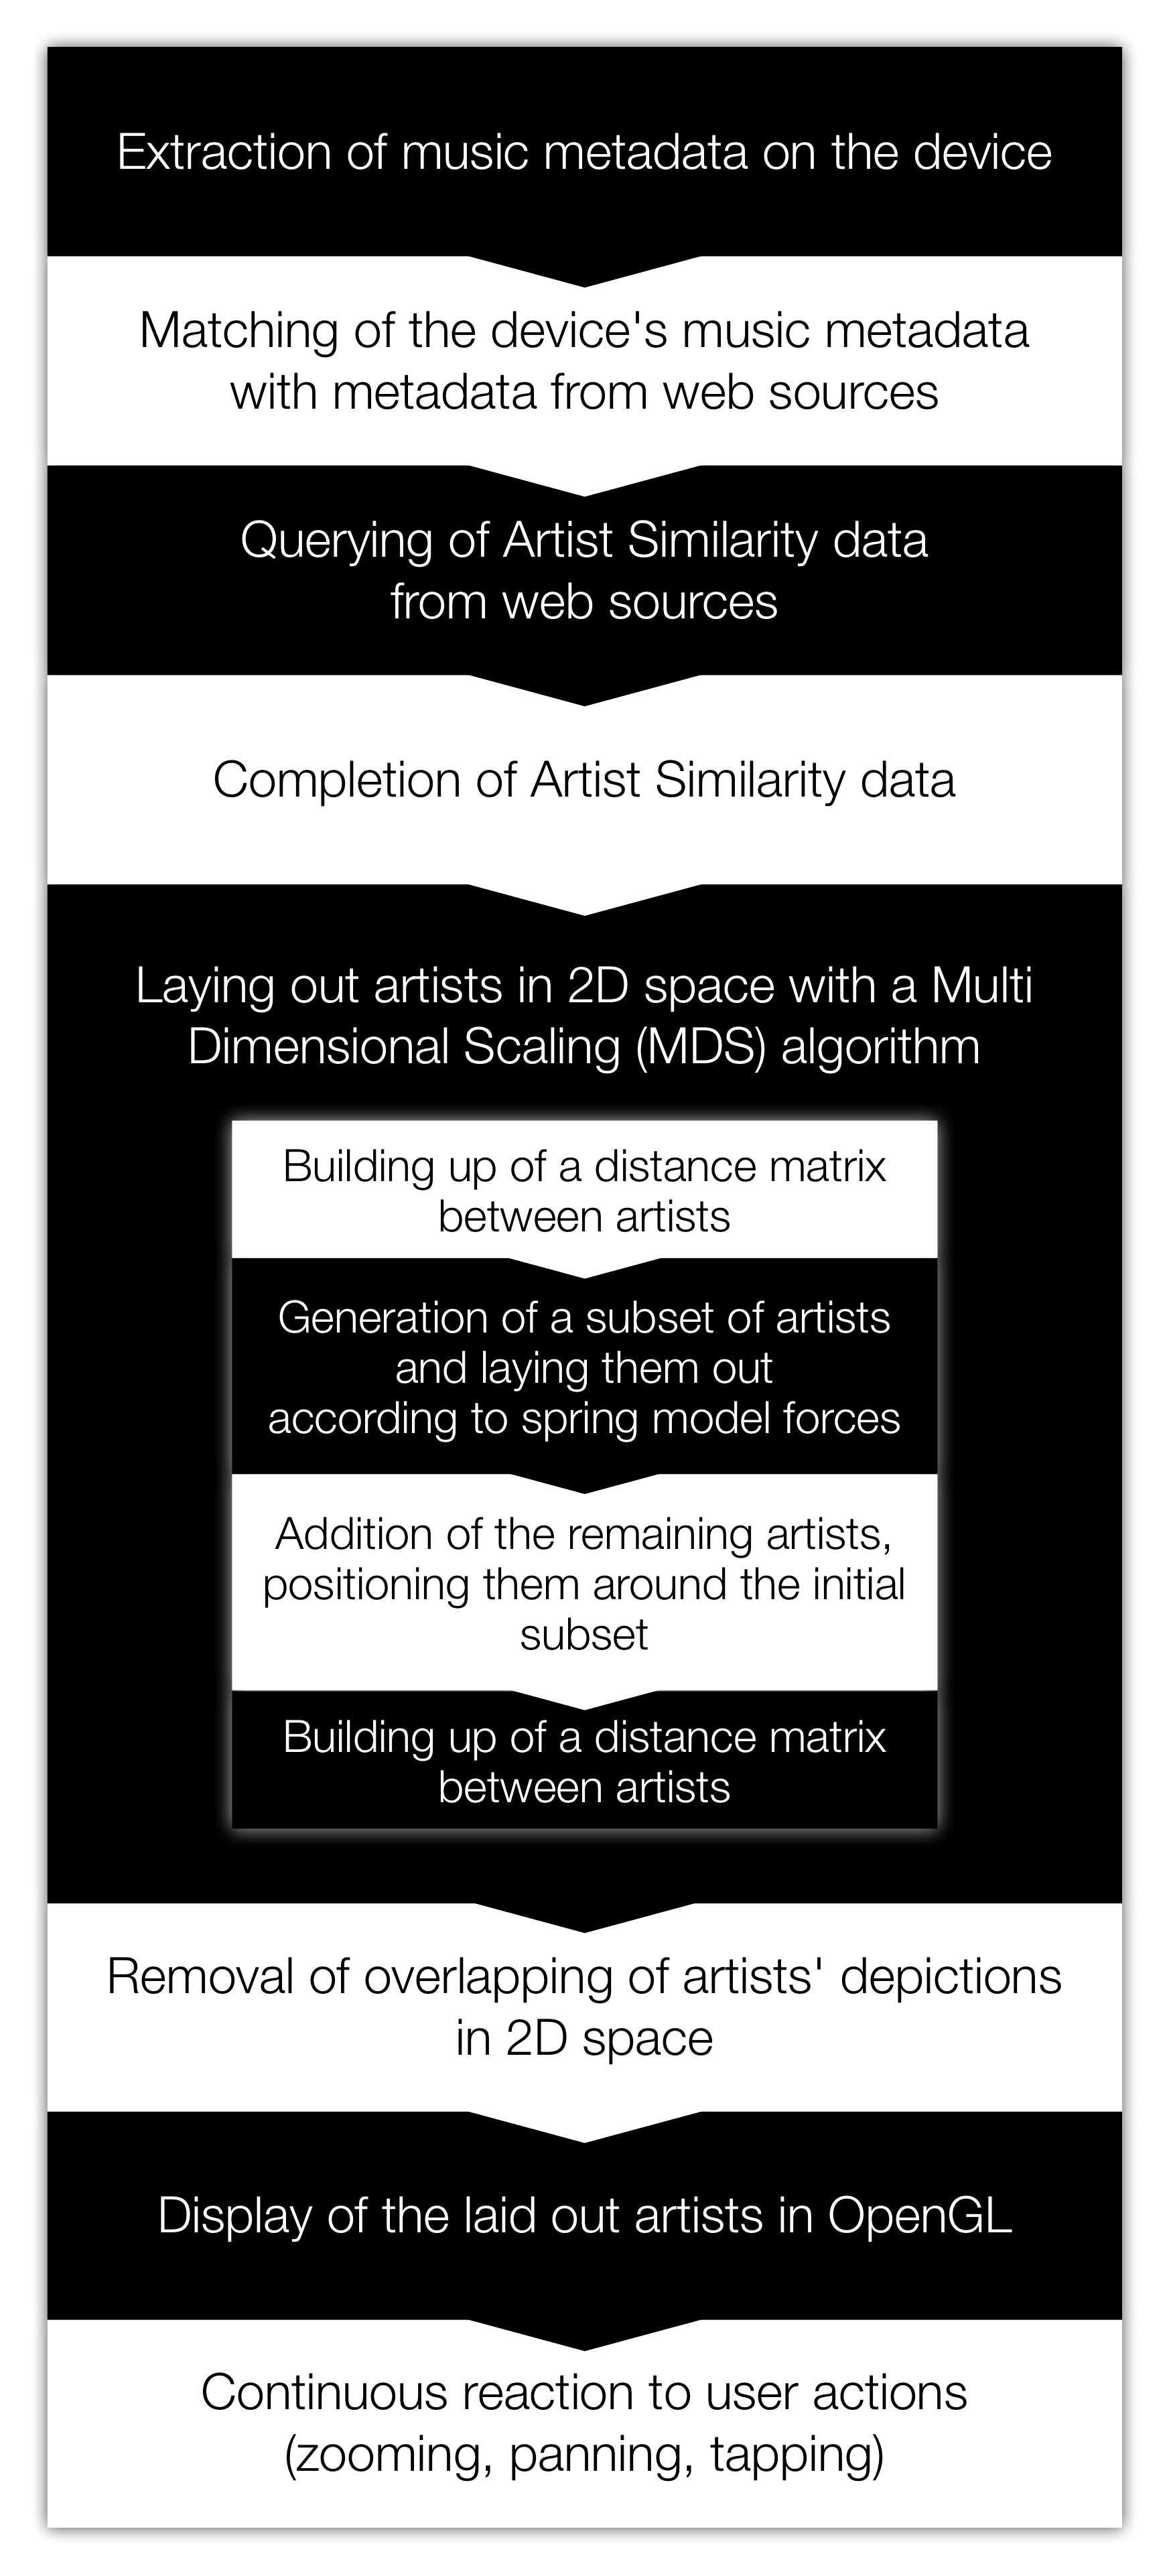
\includegraphics[width=0.45\textwidth]{figures/algorithm_flow_visualization}
  \caption{Algorithms for Library Visualization}
  \label{fig:algorithm_flow_visualization}
\end{figure}

\subsection{Artist Discovery}

Artist discovery is initiated by the user selecting a certain artist ("'subject"'), and requesting discovery mode.

\begin{figure}[H]
  \centering
    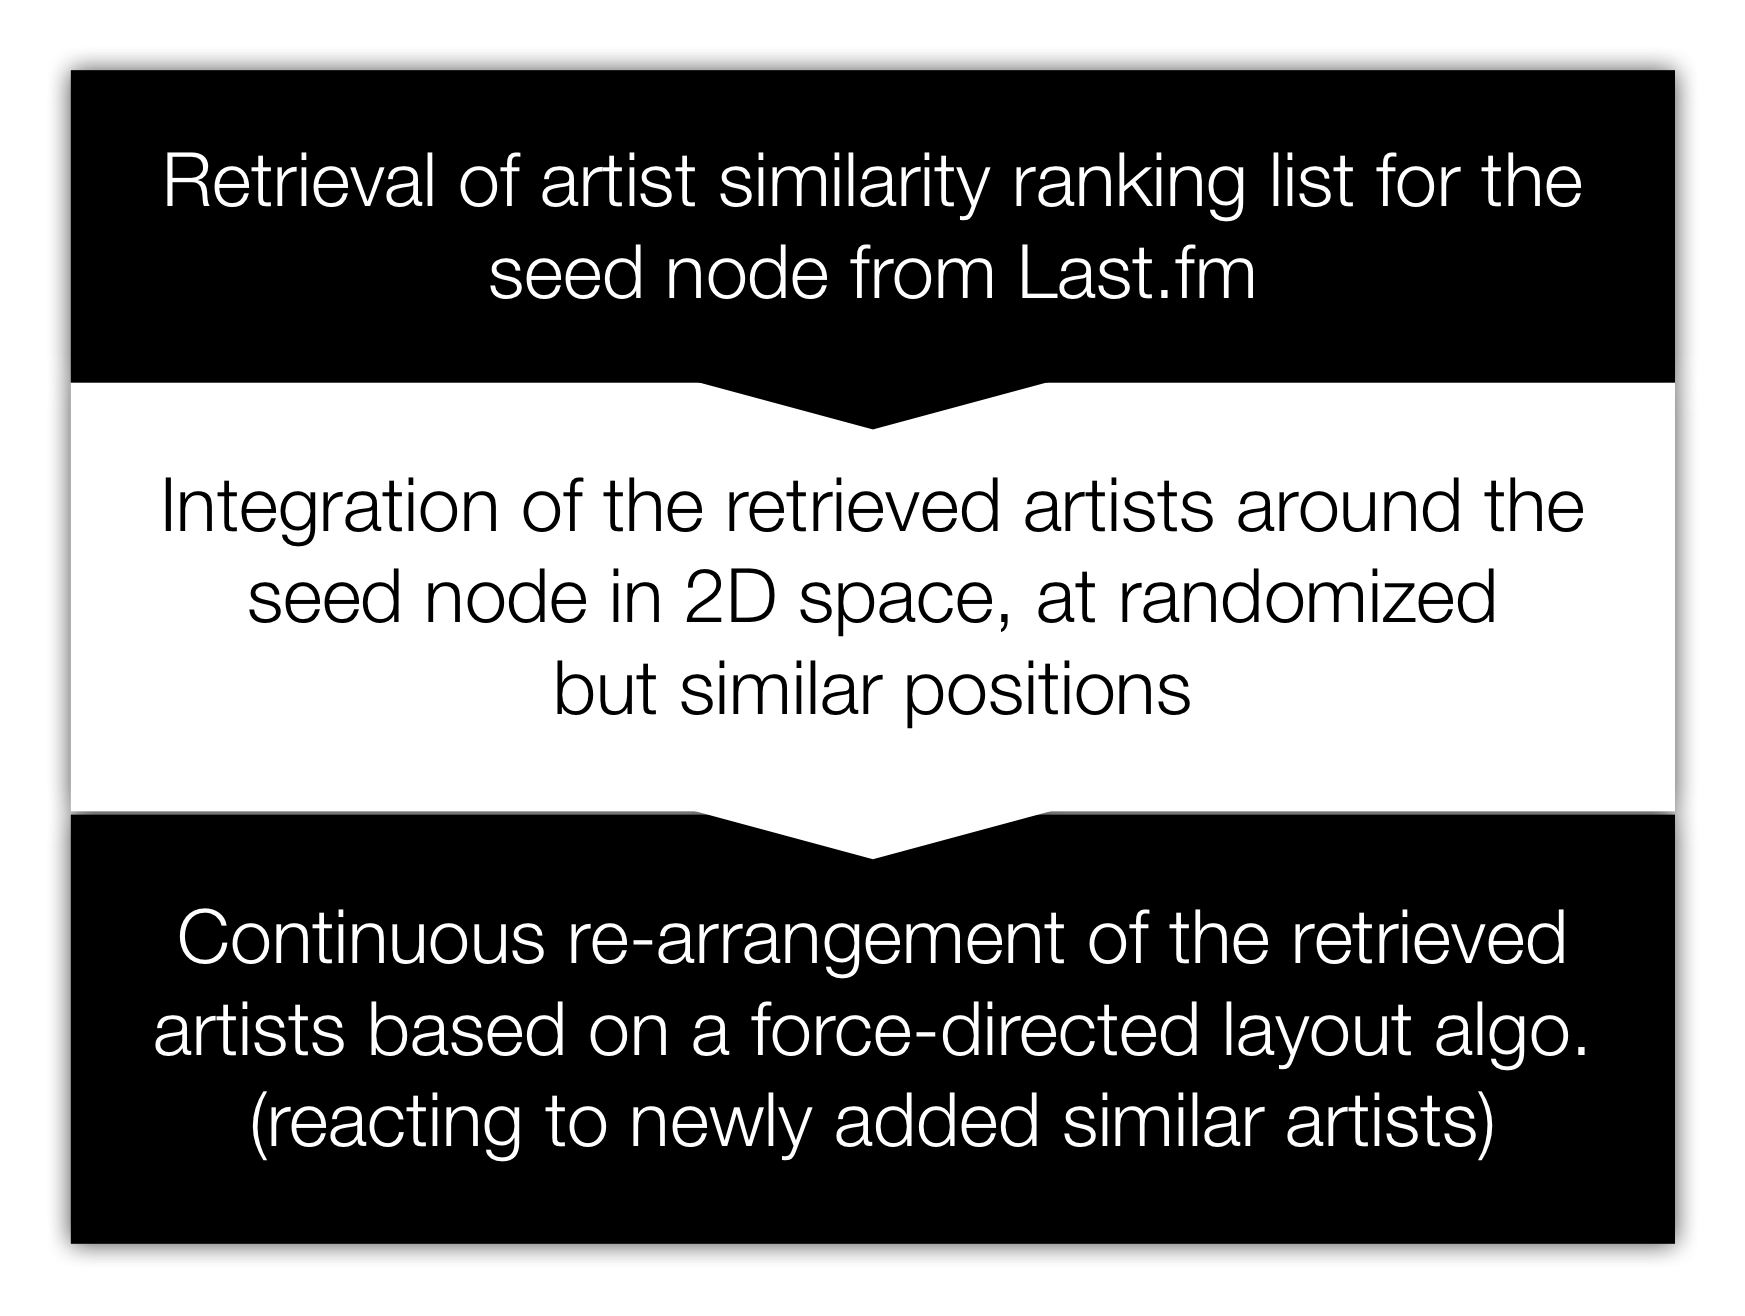
\includegraphics[width=0.45\textwidth]{figures/algorithm_flow_artist_discovery}
  \caption{Algorithms for Artist Discovery}
  \label{fig:algorithm_flow_artist_discovery}
\end{figure}

\section{Summary}

After the definition of the scope of this thesis (verification of artist similarity computational methods and implementation in a prototype), algorithms have been selected for further treatment which have already been outlined in Chapter ~\ref{ch:relatedwork}. For the computation of artist similarity, a multi-dimensional scaling method has been chosen, and the accompanying visualization is highly dependent on the computational part - therefore, a 2D visualization of the MDS output has been selected. 
While the algorithm for the removal of node overlappings in the graph resulting from the previously mentioned computation is a modification of a force-transfer algorithm, the layout computation for artist discovery has been chosen to be force-directed. Finally, an overview of the algorithms and information flow between them has been given, for both artist similarity visualization and artist discovery.
In this chapter, the computation of similarities between artists and construction of layouts based on those similarities will be presented.

\begin{itemize}
	\item \textbf {Matching of music entities from Different Sources} - Describes the methods used for merging music objects (artists, albums, titles) and their similarities, and how they deal with uncertainty regarding similarities.
	\item \textbf {Multidimensional Scaling Algorithm} - Gives details about the MDS algorithm employed for the layout of music collections.
	\item \textbf {Optimizations for Execution on Mobile Devices} - Elaborates on how aforementioned MDS algorithm can be optimized for the execution on devices with relatively low processing power.
	\item \textbf {Downsides of MDS in this Context} - Lists some downsides of the usage of MDS in the given context, as opposed to other layout methods.
\end{itemize}

\section{Matching of Music Entities from Different Sources}

In order to use similarity data from different information sources (here: web services), these data items have to be consolidated in a way that assures that they don't mix up - e.g., objects with the same name are assumed to depict the same artist (typos or naming variations should be amended).

The following approach has been chosen to perform the gathering and matching of different online sources of similarity data:

\begin{enumerate}
	\item A list of music files residing on the mobile device is compiled, and from there a list of locally available artists is generated (the list is not processed, meaning that spelling errors or duplicates are not corrected).
	\item For all locally available artists, the available online APIs are queried, returning lists of similar artists.
	\item Within the returned lists, the locally available artists are searched for - if there is a match, a
similarity connection is stored for the related artists.
\end{enumerate}

The matching itself takes place implicitly in steps 2 and 3. In step 2, the matching is performed by Web Services
itself (which is assumed to be highly optimized and reliable); in step 3, the matching happens in the form of a
case-insensitive equality-assertion (artist name equals artist name). 

The result of this approach is a number of similarity connections between locally stored artists. It can be assumed that as much as 90 percent or more of potential similarity connections cannot be established based on the web APIs' results - currently, they cannot be queried specifically for the similarity between artist X and artist Y, but this information is only available when artist Y is in artist X's similar artists list, or vice versa. Therefore, a meaningful default similarity for unknown similarities must be defined. The author has decided on a statistical approximation - any artist Y which is not in artist X's similarity list (returned by a web API) is assigned a similarity connection \{X, Y\} of \\
\emph{0.5 * [least similarity value in the list of artist X's similar artists]} (expected value).

\section{Multidimensional Scaling Algorithm}
\label{sec:mds-algorithm}



\subsection{Fitness of MDS for The Given Problem}

The subjective similarity of music, or artists in particular, can be expressed as attributes which are assigned by human beings (their opinions). Such attributes may be:

\begin{itemize}
	\item Rhythm
	\item Beats per minute
	\item Mood
	\item Popularity
	\item Genre
	\item Tuning
	\item ...
\end{itemize}

Whatever the assigned attributes are - by comparing attributes of music titles to those of other titles, a similarity measure can somehow be obtained. Every attribute then can be seen as another dimension, and every music title or artist is an object in a space of N dimensions, where N is the number of attributes assigned. Therefore, the problem of laying out music collections in two-dimensional layouts with respect to their subjective similarity can be reduced to a multidimensional scaling problem.
Since the previously mentioned web sources provide readymade similarity measures between artists, we can take a shortcut here, and remain oblivious of audio attributes such as rhythm or mood. It has not been publicized how Last.fm generates similarity information based on their users' behaviour, but it can be assumed that they use Collaborative Filtering algorithms ~\cite{Takacs:2007}, or market basket analysis ~\cite{Aggarwal99anew}. Due to the possibility of externalizing similarity data aggregation to a Web Service, a major part of spring model MDS work - the filtering and mapping of different attributes w.r.t. their impact on object similarity - is a solved problem. The similarities that are retrieved from Web Services can directly be used to calculate the length of the connecting springs.

\subsection{Concrete MDS Algorithm}

As mentioned before, the chosen MDS algorithm is based on a spring model. In the real world, steel rings interconnected with springs strive to form an equilibrium, where all forces enacted by the springs are balanced. In a perfect equilibrium, the position of every steel ring is a compromise of all forces acting on it, and the rings will not move anymore. The "'system stress"' is then zero. The real-world spring system will also produce non-perfect ending states because of energy loss in the system - at some point, the rings will not move anymore because the original kinetic energy has transformed into other forms of energy and is not available for movement of rigid springs.
In a digital emulation of this concept, objects are moved around by high-dimensional forces (springs) until, theoretically, an equilibrium has been reached. However, the balancing effect (swinging) produced by these forces cannot happen continuously as in the real word. Instead, the swinging spring effect is approximated by computing iterations, each representing a system state at a certain time. Since there is no loss of energy in the system (as observed in the real-world spring system) for every iteration, there are configurations in which the objects will be pushed around by the forces forever, never reaching a final static state. It is therefore common to limit the amount of iterations or regard the positions of objects as "'good enough"' when the system stress has fallen below a threshold. Since system stress grows proportionally to the number of objects (if stress among them stays the same), an optimal system stress threshold is non-trivial to calculate.
Research has produced both basic and more refined algorithms which approximate the behavior of a spring model. 
The most basic approach is mentioned in \cite{Chalmers:1996:LIT:244979.245035} (and then refined for faster computation) - 
it starts out by assigning coordinated in low dimensional space (2D or 3D is most likely) for each object (coordinates may be related to high dimensional coordinates, or may be randomized). Iterations are then performed on the low dimensional model, by performing these steps:

\begin{enumerate}
	\item For every object, calculate its supposed low dimensional distance (LDD) to every other object. The supposed LDD is determined by a custom function (e.g., the Euclidean distance). Here, this function takes a similarity value retrieved from web sources as a parameter.
	\subitem If the supposed LDD does not match the actual current LDD, calculate a force into a certain direction (vector), either attractive or repulsive (pulling to or pushing from each other), and save it for later application.
	\item Apply all previously saved forces onto the corresponding objects.
\end{enumerate}		

\section{Optimizations for Execution on Mobile Devices}

The most basic MDS algorithm described previously is computationally too expensive to perform with a reasonably large data set (up to 1000 objects) on a mobile device, at a complexity of $O(N^3)$ or $O(N^4)$ \cite{Chalmers:1996:LIT:244979.245035}. Chalmers therefore introduces a stochastic sampling method and the use of neighbor sets in \cite{Chalmers:1996:LIT:244979.245035}. Instead of performing force calculations for every object to every other object in each iteration, subsets of objects are picked and used randomly. Also, for every object a neighbor set is created which keeps objects of the lowest high-dimensional distances. It is reported in \cite{Chalmers:1996:LIT:244979.245035} that these optimizations reduce the algorithm's complexity to $O(N^2)$.

Further on, \cite{Morrison:2003:FMS} introduces another optimization: Initially, only a subset of all objects is selected and the aforementioned stochastic layout algorithm is performed on those. Then, the rest of the objects is added to the layout following an estimation of their best positions. Finally, the stochastic layout algorithm is performed again, for a limited number of iterations. Thus, the complexity of the algorithm is further reduced to $\mathcal O(N*\sqrt{N})$.

\subsection{Selected Algorithm in Detail}
\label{subsec:mds-selected-algorithm}

The optimized algorithm is composed of these steps (C1, C2, C3, C4 being predefined constants):

\begin{enumerate}
	\item Select a random subset of $\sqrt{N}$ objects (N = number of all objects)
	\item Perform a sampled MDS calculation on the initial layout, by performing C1 iterations of the following:
		\subitem For each object in the subset (called "'subject"') do:
			\subsubitem Generate a random subset of all objects containing C2 objects; concurrently, switch objects into subject's neighbor set if either the set has not reached its capacity, or if the object has a lower high-dimensional distance than the current most distant neighbor.
			\subsubitem For every object in either the random subset or the neighbor set, calculate its supposed low dimensional distance (LDD) to the subject. The supposed LDD is determined by a custom function (e.g., the Euclidean distance). Here, this function takes a similarity value retrieved from web sources as a parameter.
			\subsubitem If the supposed LDD does not match the actual current LDD, calculate a force for subject into a certain direction (vector), either attractive or repulsive, and save it for later application. (Note: Only the subject is moved)
		\subitem Apply all previously saved forces onto the corresponding subjects.
	\item For every object (called "'subject"') NOT in the initial subset do (subset Z containing all objects from the initial subset):
		\subitem Find the most similar (lowest high-dimensional distance) object in Z, and choose the best quadrant around it, to place the subject there. (There are four quadrants surrounding the most similar object, top-left, top-right, bottom-left, bottom-right.)
			\subsubitem Vectors are constructed from the most similar object to each quadrant's center, with a length corresponding to the similarity between the two objects.
			\subsubitem Positioning tests are performed by moving the subject to the end of each constructed vector, and calculating the stress between the most similar object and the temporarily moved subject. The vector of the quadrant which yields the lowest stress wins the test, and subject is assigned the resulting position, which is again the result of adding the vector to the most similar object's position.
		\subitem Improve on subject's new position by performing C3 iterations very similar to step 2., but only with the initial subset of objects.
		\subitem Add subject to Z.
	\item Perform a sampled MDS calculation like in step 2. with C4 iterations, but with all available objects instead of only the initial subset. The purpose is to move grossly mispositioned objects to a better position - very good results can be achieved with a low number of iterations (C4).
		
\end{enumerate}

\section{Downsides of MDS in This Context}

The advantages of MDS have been described sufficiently in this section. However, there are some downsides to this approach too, some of which are inherent to the problem at hand and which could not be alleviated by using another method.

If the internal structure of the transformed music entity set \textbf{is not expressible in a two-dimensional space without tradeoffs}, the spatial distances between entities will not always depict their similarity correctly. The larger the transformed set is, the more will the entities' 2D distances be different from their expected ("'should be"') distances. It can be viewed as a given that in most cases distances between some entities will not at all match their expected lengths.

The layout produced by the aforementioned MDS method \textbf{will never be the same for two different calculations}, since many parts of the algorithm involve randomness 
\footnote{The introduction of randomness in the layout creation algorithm has been necessary, as mentioned before, because it reduces its time complexity from $O(n^3)$ or even $O(n^4)$ to $\mathcal O(N*\sqrt{N})$. Without these optimizations, the algorithm would hardly be able to produce a layout in a mobile app in reasonable time.}.
While the addition of some entities is possible after the layout has been completed, a complete rerun of the algorithm will become necessary if similarities change. This is suboptimal for users because they have to reorient themselves after every major layout change.

The MDS method presented earlier in this chapter relies on definite high-dimensional vectors (from which similarity measures can be derived), which is not available here - in the context of computing similarity based on web sources, it is unlikely that a similarity measure can be found for every entity-entity relationship. Therefore, \textbf{estimations have to be used for unknown similarity relationships}, potentially polluting the calculation with incorrect values.

\section{Summary}

The matching of music entities from various sources has been described as a simple, straightforward process, and it was also mentioned how calculation of expected values can provide meaningful approximations for unknown similarities between artists. Subsequently, an introduction to multidimensional scaling and the simplest possible MDS algorithm was given. 

Optimizations which make execution of such a computation for a reasonable number of objects possible on a current mobile device have then been specified, namely the introduction of sampling and interpolation. Finally, downsides of the application of MDS for the generation of layouts were found - layouts would hardly ever look the same after two separate calculations, and estimations of unknown artist similarities may pollute the resulting layout.
In this section, the visualization of objects whose positions have previously been computed (see section ~\ref{ch:computation}) will be discussed. Also, the interaction patterns for the mobile application prototype will be defined.

INSERT SUBCHAPTERS LIST HERE

\section{Visualization}

After the computation of similarity measures and the resulting layout of music objects has been performed (see section ~\ref{ch:computation}), the mode of visualization has to be defined. As has already been discussed, the possible modes of information display have been narrowed down due to several constraints, determining that the visualization must be two-dimensional. Small screens on mobile devices introduce a further constraint: in most use cases, not all of the content will fit on one screen; therefore, a zooming and panning mechanism will be employed. To provide users with a rich experience, the objects shall not be shown as points, but as shapes - if an image of the object exists in an online source, it shall be used, or otherwise, an arbitrary rectangle shall be shown. In order that users can orient themselves better, a non-solid background will be used - ideally, it will emulate 3-dimensionality by moving and zooming while the user pans or zooms the graph.

\section{User Interaction}

Information will be displayed to the user in a hierarchical way - to limit the amount of information displayed all at once, it is split up and logical links are established. The hierarchy is made up of:

\begin{itemize}
	\item \textbf{Artists} - images and labels of the respective artists are displayed. Their positions relative to each other depict the artists' similarities. Here, the user can select an artist and proceed to the next hierarchical level by pressing a button:
	\item \textbf{A certain artist and her album(s)} - images and labels of the previously selected artist and her albums (stored on the device), arranged in a starlike way (without any similarity information conveyed). Again, the user can select an album and proceed to the next hierarchical level by pressing a button:
	\item \textbf{An album's tracks} - a list of tracks, carrying the image of the belonging album. The user can choose to start playback of one or all of the tracks.
	\item \textbf{Related Artists (Discovery)} - From within the \textbf{Artists} view, the user can choose to display artists which are related to a certain artist in a semantic way, as established by the Last.fm API.
	
\end{itemize}

To improve the user's understanding of the current navigational status, so-called breadcrumbs. Breadcrumbs achieve "'visitor location awareness in a simple and direct way"' \cite{Tesoriero:2008:Breadcrumbs} if applied to 2D spaces. A breadcrumb in this context is a series of links displayed on top of the graph, each representing one hierarchical level. An example for breadcrumbs shown while a list of tracks (lowest hierarchical level) could be: "'Artist: Air > Album: Talkie Walkie"'. Further, a button is added which positions the viewport at the center of the graph, for the user to recover in case she has lost track of the viewport's position.

Within the graph viewport, interaction will be a mix of touch based interaction and hardware buttons, since most Android devices provide those affordances. Special accessibility functions for interaction without touch gestures are omitted since they would go beyond the scope of this thesis.
Following the established conventions of touch interfaces, navigatable objects (like artists or albums) are made touchable. Likewise, the user can reach upper view hierarchies by pressing the hardware (or software-emulated) back button common to Android devices.
Exploration of the graph is performed by two common touch gestures, namely pinch-to-zoom and one-finger-panning. To zoom, the user places two fingers on the graph viewport and moving her fingers either apart (zooming in) or towards each other (zooming out). To pan, the user places one finger on the graph and moves it around as if it were a piece of paper and the screen an aperture showing the paper.

\section{Removal of Node Overlapping}

As the reader may have noticed, the positions of objects computed as described in section ~\ref{ch:computation} don't respect any aesthetic criteria. ~\cite{Li:2005} gives an overview of such criteria, three of which also apply to graphs produced by MDS:

\begin{itemize}
	\item Minimisation of the area taken up
	\item Minimisation of total object distance
	\item Aspect ratio close to or matching the specification
\end{itemize}

However, an even more important aesthetic factor in the perception of graph drawings is the \textbf{removal of node overlappings}. The computational layout method applied in this thesis - spring model MDS (see section ~\ref{ch:computation}) - can not give any heed to overlapping nodes (or margin between them), since nodes are positioned as points, not 2D objects. However, the objects do need to be displayed as 2D shapes (e.g. as rectangles, circles, images,...), and therefore the resulting layout can (and in many cases, will) contain overlappings.
As this may impact the perception of the graph by humans in a negative way (objects may even be completely hidden by other objects), a way has to be found to eliminate overlappings as reliably as possible, without affecting the conveyed information of object similarities too much.

The authors of ~\cite{journals/vlc/MisueELS95} therefore define the concept of the Mental Map, meaning that a graph has properties which should be maintained if transformed: Orthogonal Ordering, Proximity Relations, and Topology. An algorithm called Force Scan (FS) is then proposed to remove node overlappings while preserving the Mental Map of a graph. FS operates by first moving nodes horizontally, maintaining their horizontal ordering, and then moving nodes vertically, maintaining their vertical ordering. Several improvements to FS have been discussed (~\cite{Hayashi:1998:LAP:647550.728930} ~\cite{Huang03force-transfer:a} ~\cite{Li:2005}), while the algorithm in ~\cite{Huang03force-transfer:a} - \textbf{Force Transfer (FT)} - seems to be the most suitable for this thesis' use case, as it is of lower computational complexity than FS and produces pleasing layouts.

The FT algorithm identifies clusters of overlapping nodes, and then performs transfer scans on them: left-to-right, right-to-left, upside-to-downside, and downside-to-upside. During the scans, the nodes in each cluster are moved such that the clusters become free of overlaps. Multiple iterations may be necessary, as the separation of one cluster may cause nodes to move on top of nodes from other clusters - thereby forming new clusters. Finally, the layout eventually is overlap-free, preserving the aforementioned mental map of the graph.

The aforementioned methods of overlap-removal are complex (considering the need to form clusters), so the author decided to employ a more basic approach, but very similar to the previous algorithms. The graph canvas is virtually emptied, and re-filled one by one with the originally contained artist nodes, while making sure that a newly added node does not overlap with any others. The algorithm is described in the following listing:

\begin{enumerate}
\item Remove all nodes from the graph structure.	
\item For every node ("'subjectNode"') do:
	\subitem For every node ("'alreadyPositionedNode"') in the set of already positioned nodes do:
	\subsubitem If the distance between subjectNode and alreadyPositionedNode is beneath a
	threshold, create a vector from alreadyPositionedNode's center to subjectNode's center, set
	its length such that they don't overlap, and displace subjectNode by it.
	\subsubitem If subjectNode still overlaps with another node, step to 2.1.
	\subsubitem Add subjectNode to the set of already positioned nodes.
\end{enumerate}

\section{Summary of this Section}
One of the objectives of this thesis is the implementation and analysis of a prototype App for mobile devices. In this chapter, the previously selected algorithms will be put into the context of the App's implementation, and the App's structure itself will be detailed. This chapter is structured as follows:

\begin{itemize}
	\item \textbf {About Android Apps} - An introduction to the Android operating system.
	\item \textbf {Assembly of Algorithms and Information Flow In Concrete Implementation} - Gives details on algorithms and information flow between them, as previously listed in an overview in Chapter ~\ref{ch:scenario}.
	\item \textbf {Illustrations of Algorithm Steps} - Lists illustrations and descriptions of the algorithm succession in the App prototype.
	\item \textbf {Retrieval of Music Metadata} - Describes how music metadata is retrieved from a mobile device's storage and from web sources.
	\item \textbf {Retrieval of Similarity Data} - Describes how artist similarity data is retrieved from web sources, and how unknown values are approximated.
	\item \textbf {Implementation of Multidimensional Scaling} - Contains a pseudo-code listing of one step in the MDS algorithm.
	\item \textbf {Implementation of Removal of Node Overlappings} - Contains a pseudo-code listing of the algorithm implementation which removes overlappings of graph nodes.
	\item \textbf {Visualization Details} - Features implementation details of the prototype concerning visualization of graph data.
	\item \textbf {Structure of the App} - Presents the structure of the prototypical App, together with information about the target operating system.
\end{itemize}

\section{Assembly of Algorithms and Information Flow In Concrete Implementation}
\label{sec:algorithm-assembly}

In Chapter ~\ref{ch:scenario}, an overview was given of how algorithms work together in the system. In-depth implementation-specific details of this assembly and information flow will now be given. These steps are in part also illustrated in Fig. ~\ref{fig:screen_mds_1_initial} to Fig. ~\ref{fig:screen_mds_10_after_all_uncollided_nodes}.

\subsection{About Android Apps}

Android is a mobile operating system developed by the Open Handset Alliance ~\cite{url:openhandsetalliance}, led by Google. Its architecture allows for 3rd party programs (called "'apps"') to easily be run and debugged on Android devices.
Android apps are run in the Dalvik VM \footnote{A Virtual Machine (VM) is the emulation of computing hardware on which software can be run which is tailored to the emulated architecture, without ever owning the actual hardware. Virtual Machines are usually executed as programs on a host operating system. Android's Dalvik VM allows to execute computer code without the need to compile it up front, like the Java VM, from which it is derived.} which makes use of a register-based architecture, relying on a Linux kernel for low-level functionality ~\cite{dalvik}. The most wide-spread programming language for building Android apps is Java, but various other languages such as Scala or even scripting languages like Groovy or Lua can be used. Since mid 2009, developers can also write and integrate native C and C++ code by making use of the Native Development Kit (NDK).

From an app developer's perspective, the frameworks contained in Android dictate a user-centric application structure, made up of so-called Activities ~\cite{url:androidactivity}. Every Activity encapsulates a screen which is presented to the user. Activities are loosely coupled, allowing only serialized objects and primitive values to be passed between them.

User interface composition in Android is performed partly in the CPU (e.g., in Java code), and partly in the device's GPU (by using the OpenGL interface). Apps can also choose between these composition variants.

Android is a strictly touch-centric operating system, meaning that most user interactions are performed via the device's touch screen. Originally, Android devices were bound to provide hardware buttons, but starting with Android 4.0, those buttons are gradually replaced with software buttons (displayed on the touch screen).

This prototype is built and tested with Android 4.0.

\subsection{Library Visualization}

\begin{itemize}
	\item Extraction of music metadata on the device \\\\
			\textbf{Input:} Access to a data store containing the device's music library metadata. \footnote{The app prototype utilizes a standard SQLite database in order to store data which can be persisted in order to reduce computation time, thus improving the user experience.}
			  \\
			\textbf{Algorithm:} Iterates through all artists and tracks in the device's music library.
			If an entity has not yet been registered in the app's database, parts of its metadata are 
			compiled and put into the database. \\
			\textbf{Output:} Local music metadata stored in the app's database.\\
			
	\item Matching of the device's music metadata with metadata from web sources \\\\
			\textbf{Input:} Local music metadata stored in the app's database.  \\
			\textbf{Algorithm:} Iterates through all local music metadata previously retrieved (artist, albums, titles...), and calls
			Last.fm's and Echonest's RESTful API to find matching entities - picking the first match as best match. These pieces
			of remote metadata are then stored in the app's database. \\
			\textbf{Output:} Remote music metadata stored in the app's database. \\
			
	\item Querying of Artist Similarity data from web sources \\\\
			\textbf{Input:} Local music metadata and matched metadata from remote web sources stored in the app's database. \\
			\textbf{Algorithm:} Iterates through all local and remote music metadata previously retrieved, and calls
			Last.fm's RESTful API to get the 100 most similar artists for each artist in the local database. \\
			\textbf{Output:} Artist similarity relations stored in the app's database. \\
			
	\item Completion of Artist Similarity data \\\\
			\textbf{Input:} Artist similarity relations stored in the app's database. \\
			\textbf{Algorithm:} Iterates through the previously retrieved artist similarity relations, and
			adds approximations for similarity relations which have not been found in the web API's results.
			These approximations are calculated as described in Section ~\ref{ch:computation}. \\
			\textbf{Output:} Complete artist similarity relations stored in the app's database. \\
			
	\item Laying out artists in 2D space with a Multi Dimensional Scaling (MDS) algorithm \\\\
			\textbf{Input:} Complete artist similarity relations stored in the app's database.   \\
			\textbf{Algorithm:} Applies a multistep (see sub-steps) algorithm which uses previously
			retrieved similarity data to position nodes resembling artists without overlappings.  \\
			\textbf{Output:} Graph structure of nodes resembling artists, laid out such that their position 
			indicates their similarity to each other. \\
			
		\begin{itemize}
			
			\item Building up of a distance matrix between artists \\\\
				\textbf{Input:} Complete artist similarity relations stored in the app's database. \\
				\textbf{Algorithm:} Iterates through all artist similarity relations, calculates a
				distance value (\emph{d = 1 - Similarity}, d $\in$ [0, 1], Similarity $\in$ [0, 1]), and writes it into
				a matrix data structure where both dimensions' labels consist of all existing artists. \\
				\textbf{Output:} Distance matrix of artists, based on their inverted similarities. \\
				
			\item Generation of a subset of artists and laying them out according to spring model forces	\\\\
				\textbf{Input:} Distance matrix of artists, based on their inverted similarities. \\
				\textbf{Algorithm:} Picks a random sample of artists of size $\sqrt{N}$ (N: number of all artists), assigns random positions to them,
				and applies a multi-dimensional scaling algorithm on them (see subsection 
				~\ref{subch:implementation-mds} later in this section). \\
				\textbf{Output:} Graph structure of nodes resembling artists (correctly positioned subset) \\
				
			\item Addition of the remaining artists, positioning them around the initial subset \\\\
				\textbf{Input:} Graph structure of nodes resembling artists (correctly positioned subset) \\
				\textbf{Algorithm:} Iterates through the remaining artist nodes and positions each on a position
				in the vicinity of its most similar artist (estimating which quadrant will be the best, as described in Chapter ~\ref{ch:computation}). \\
				\textbf{Output:} Graph structure of nodes resembling artists, many of them suboptimally positioned \\
				
			\item Application of spring model forces on all nodes for a few iterations \\\\
				\textbf{Input:} Graph structure of nodes resembling artists, many of them suboptimally positioned \\
				\textbf{Algorithm:} Applies the aforementioned multi-dimensional scaling algorithm on the whole graph of
				all artist nodes, thus reducing system stress \footnote{System stress is a metric for how well the current layout of a graph satisfies its internal forces. The higher the disconnect between the node's optimal distances and their actual distances is, the higher is the stress. One way to calculate stress is: S = $\sum_{n_i, n_j}^{n_N} ( Actual Distance(n_i, n_j) - Optimal Distance(n_i, n_j) ) ^ 2, n_i != n_j$} (finding a better position for each artist).  \\
				\textbf{Output:} Graph structure of nodes resembling artists, laid out such that their position 
				indicates their similarity to each other.\\
				
			\end{itemize}
				
	\item Removal of overlapping of artists' depictions in 2D space	\\\\
				\textbf{Input:} Graph structure of nodes resembling artists, laid out such that their position 
				indicates their similarity to each other. \\
				\textbf{Algorithm:} Empties out the graph, and re-adds the artist nodes back into it, one by one,
				while optionally moving nodes when they are added such that they do not overlap any other nodes. This
				movement is determined by the vector of both nodes' center coordinates and their amount
				of overlapping. For more details about this algorithm, see 
				~\ref{subch:implementation-overlapping} later in this section. \\
				\textbf{Output:} Graph structure of nodes resembling artists, laid out such that they don't 
				overlap each other and their position indicates their similarity to each other. \\
				
	\item Display of the laid out artists in OpenGL	\\\\
				\textbf{Input:} Graph structure of nodes resembling artists, laid out such that they don't 
				overlap each other and their position indicates their similarity to each other. \\
				\textbf{Algorithm:} Displays the graph on an OpenGL canvas (3D), by using the artists' images (in form
				of textures) and their names (rendered to textures). Sets the viewport and transformation
				matrices such that a 2D view is simulated, displaying artist nodes as viewed from above. \\
				\textbf{Output:} OpenGL view object and auxiliary system objects \\
				
	\item Continuous reaction to user actions (zooming, panning, tapping) \\\\
				\textbf{Input:} OpenGL view object and auxiliary system objects. \\
				\textbf{Algorithm:} Continuously reacts to user interface inputs, by moving the OpenGL canvas'
				pseudo-camera (i.e., manipulating the model transformation matrix) for zooming and panning.
				Marks an artist node as selected when the user taps onto it, and displays a context menu. \\
				\textbf{Output:} Updated view state
\end{itemize}

\subsection{Artist Discovery}

\begin{itemize}
	\item Queries last.fm for the N artists most similar to "'subject"'\\\\
				\textbf{Input:} "'Subject"' artist the user has selected for discovery. \\
				\textbf{Algorithm:} Queries Last.fm for the artists most similar to "'subject"', and returns
				an excerpt of those. \\
				\textbf{Output:} Excerpt of artists most similar to "'subject"'. \\
	\item Integration of the retrieved artists around "'subject"' in 2D space, at randomized but similar positions \\\\
				\textbf{Input:} Excerpt of artists most similar to "'subject"'. \\
				\textbf{Algorithm:} Applies a force-based layout algorithm on the collection of "'subject"' and
				its similar artists, such that the similar artists are arranged in a star around "'subject"'. \\
				\textbf{Output:} Graph structure of nodes resembling artists, laid out such that similar
				artists encircle "'subject"'. \\
	\item Continuous re-arrangement of the retrieved artists based on a force-based layout algorithm (also reacting to newly added similar artists) \\\\
				\textbf{Input:} Graph structure of nodes resembling artists, laid out such that similar
				artists encircle "'subject"'. \\
				\textbf{Algorithm:} As the user selects more artist nodes as "'subject"' and load
				its similar artists, this algorithm is then restarted, but the previous subjects and their
				similar artists are kept, and their positions adapted as needed - i.e., force-based layout
				calculation does not stop for those. \\
				\textbf{Output:} Updated graph structure of nodes resembling artists, laid out such that similar artists encircle "'subject"', also related to previously retrieved similar artists \\
\end{itemize}

\section{Illustrations of Algorithm Steps}

The previously described algorithms used for the composition of the App will in the following be  illustrated by screenshots of their outcome. These screenshots are based on an example library which the author of this thesis used while implementing, debugging, and testing the App. Many of the states depicted on the screenshots are not to be found in the actual App, because during the computational algorithms the current graph state is hidden from the user. Only Figure ~\ref{fig:screen_mds_10_after_all_uncollided_nodes} is a screenshot of the final version of the App. The other figures serve as pure illustration for this thesis.

\subsection{Before the Computation}

In figure ~\ref{fig:screen_mds_1_initial}, the initial graph state is shown - a loose collection of artist nodes strewn around the graph's origin in a random manner. At this point, no computation has yet been performed except the assignment of random positions (to avoid edge cases during the application of spring model forces later on, which arise when all nodes are located at the origin).

\begin{figure}[H]
  \centering
    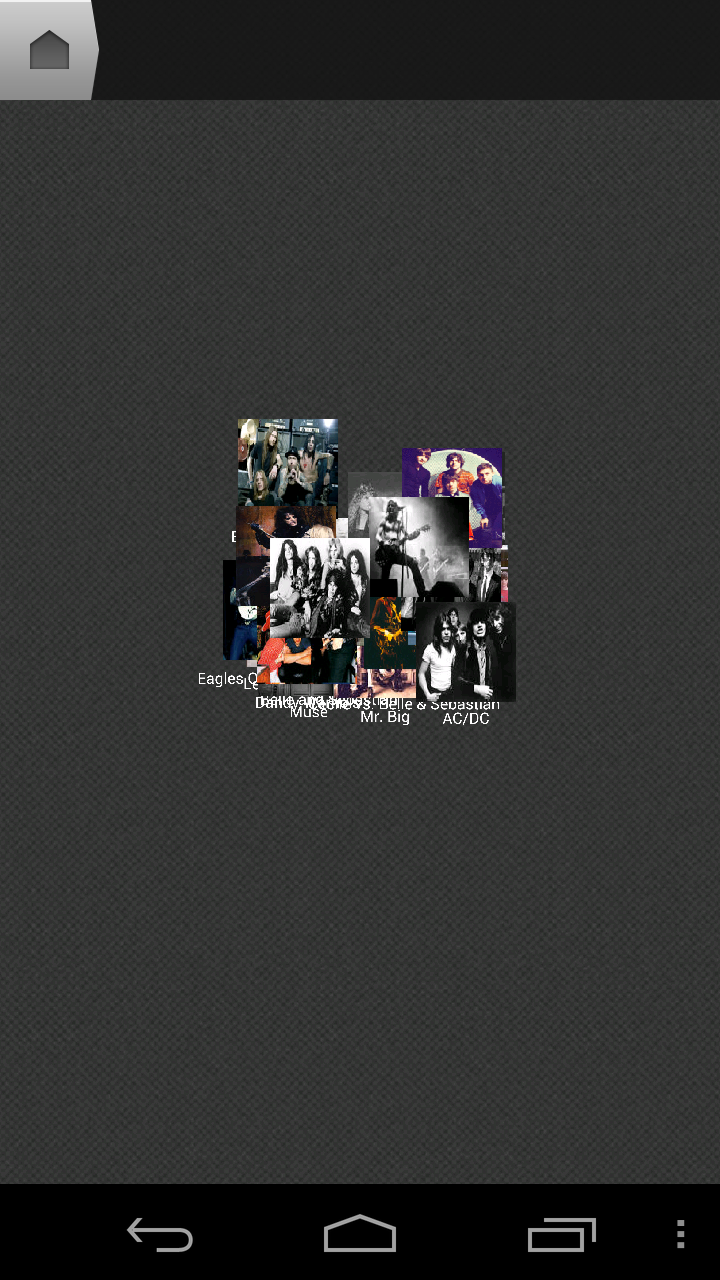
\includegraphics[width=0.4\textwidth]{figures/screen_mds_1_initial}
  \caption{The initial graph state before MDS calculation}
  \label{fig:screen_mds_1_initial}
\end{figure}

\newpage
\subsection{After 5 Subset Iterations (MDS)}
\label{subsec:mds-after-five-subset-iterations}

As previously described in sections ~\ref{sec:mds-algorithm} and ~\ref{sec:algorithm-assembly}, the first steps in the App's MDS computation are:

\begin{enumerate}
	\item Generation of a subset of nodes, and
	\item Application of a number of spring model iterations on this subset.
\end{enumerate}

The screenshot depicted in figure ~\ref{fig:screen_mds_2_after_5_subset_iterations} shows the graph's state after five iterations of step 2. If compared to figure ~\ref{fig:screen_mds_1_initial}, it can be observed that four of the artist nodes have been moved to more outward positions.

\begin{figure}[H]
  \centering
    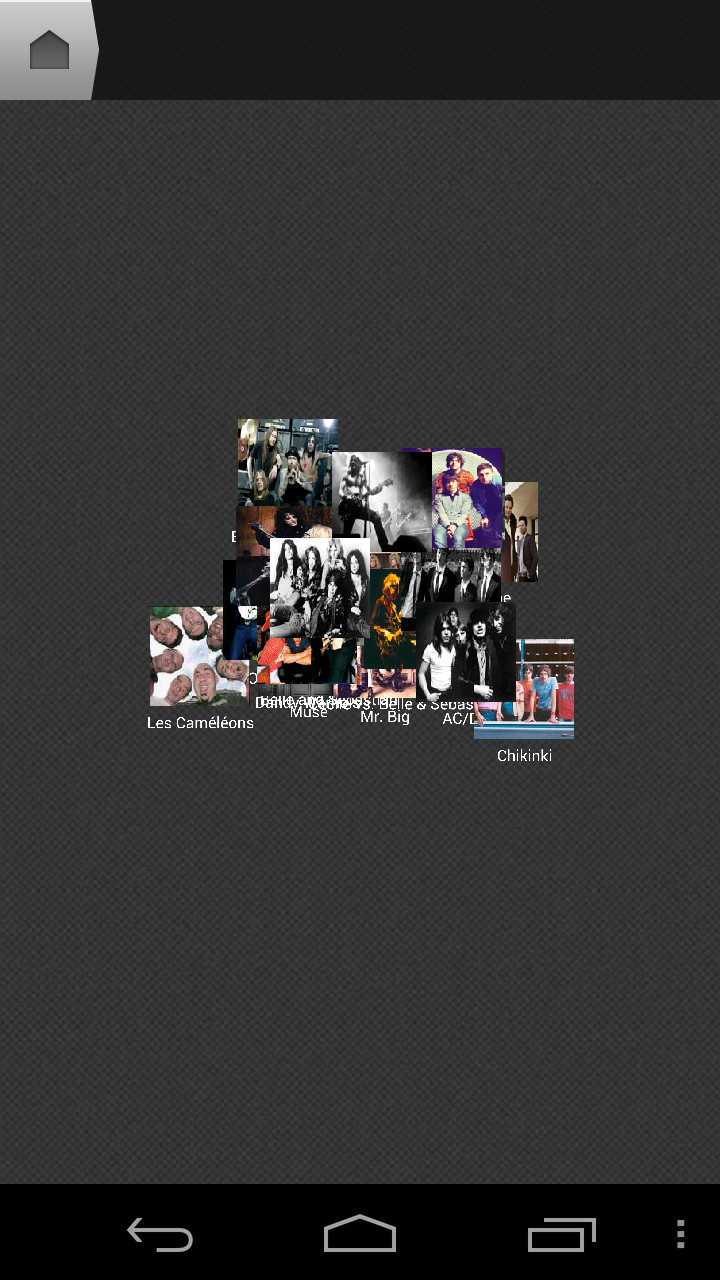
\includegraphics[width=0.4\textwidth]{figures/screen_mds_2_after_5_subset_iterations}
  \caption{Graph state after 5 iterations of the initial subset}
  \label{fig:screen_mds_2_after_5_subset_iterations}
\end{figure}

\newpage
\subsection{After 20 Subset Iterations (MDS)}

Similar to the previous figure, the following screenshot ~\ref{fig:screen_mds_3_after_20_subset_iterations} shows graph state during the second step (application of a number of spring model iterations on the initial subset) of MDS computation, but with 20 iterations of progress. It's easy to see that the four artist nodes (which have already been moved in figure ~\ref{fig:screen_mds_2_after_5_subset_iterations}) have been displaced even more.

\begin{figure}[H]
  \centering
    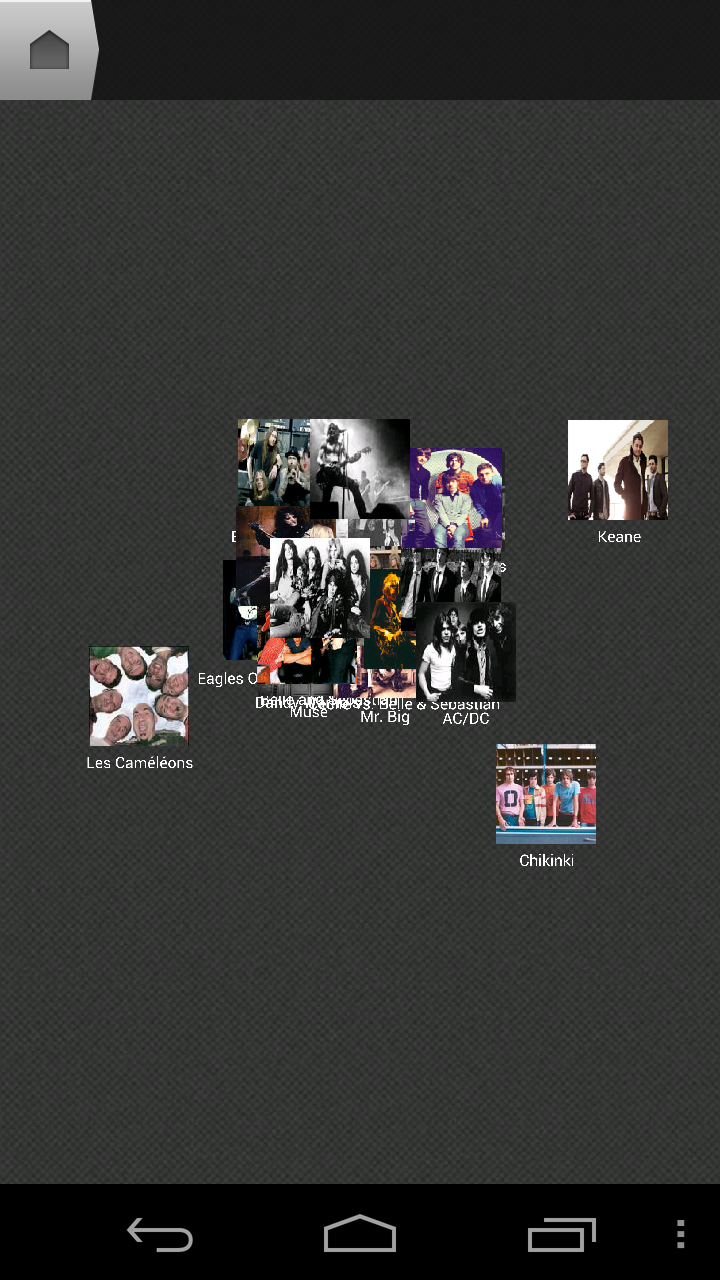
\includegraphics[width=0.4\textwidth]{figures/screen_mds_3_after_20_subset_iterations}
  \caption{Graph state after 20 spring force iterations of the initial subset}
  \label{fig:screen_mds_3_after_20_subset_iterations}
\end{figure}

\newpage
\subsection{After Placements of 5 Remaining Nodes (MDS)}

After spring model forces have been applied to the initial node subset, the remaining nodes (not being in the initial subset) are now placed in semantically sane positions. In figure ~\ref{fig:screen_mds_4_after_5_restnode_additions}, it can be observed that some nodes visible on the screen have been moved to positions which differ greatly from the old positions in the last screenshot. Because the placement algorithm is of low complexity, as has been shown in Section ~\ref{subsec:mds-selected-algorithm}, placements are performed in much shorter time than the previously described subset iterations.

\begin{figure}[H]
  \centering
    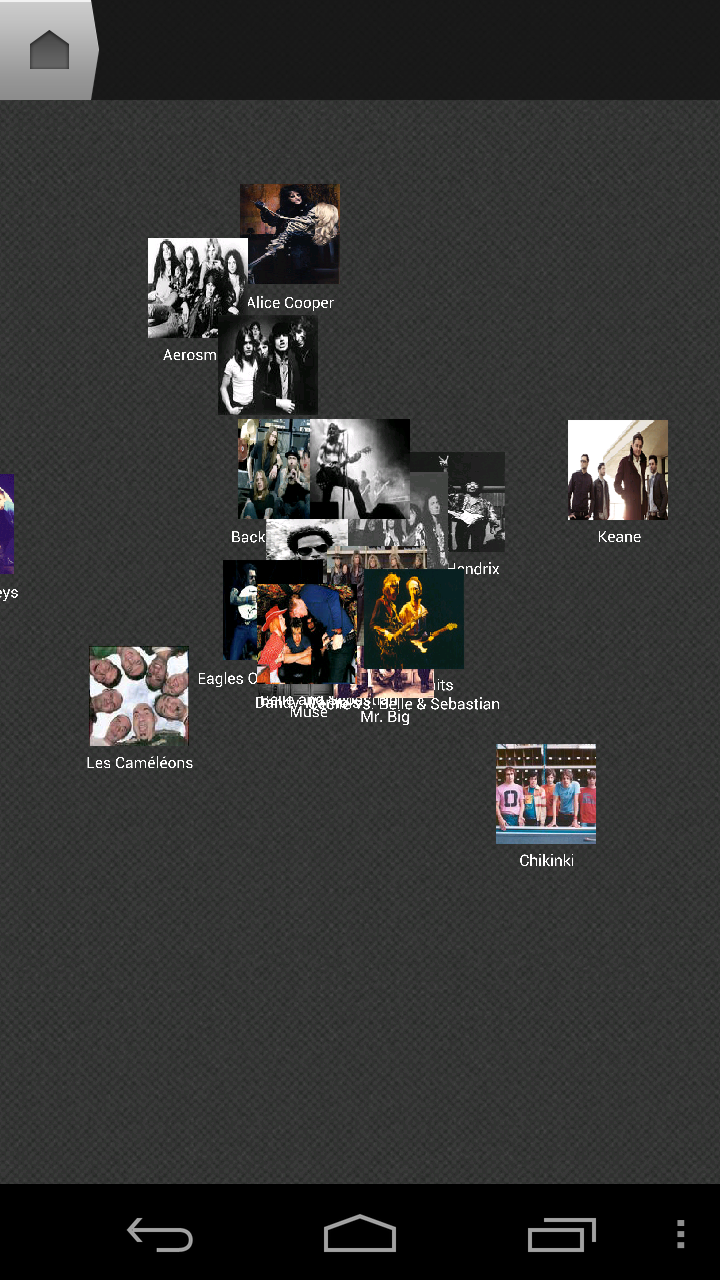
\includegraphics[width=0.4\textwidth]{figures/screen_mds_4_after_5_restnode_additions}
  \caption{Graph state after 5 placements of nodes outside the initial subset}
  \label{fig:screen_mds_4_after_5_restnode_additions}
\end{figure}

\newpage
\subsection{After Placements of All Remaining Nodes (MDS)}

Figure ~\ref{fig:screen_mds_5_after_all_restnode_additions} shows the graph's state after all nodes not in the initial subset have been placed in approximated positions. Although all nodes have been displaced at least once, this is an intermediate state, not yet resembling the algorithm's final outcome. Most nodes should be at least near their optimal position, minimizing system stress, but tests have shown that some nodes will be displaced by much in the following placement corrections. Due to the nature of the performed placement approximation, the such placed nodes take into account only the most similar node - yet there may be other nodes at an entirely different position in the graph to which the placed node is also similar.

\begin{figure}[H]
  \centering
    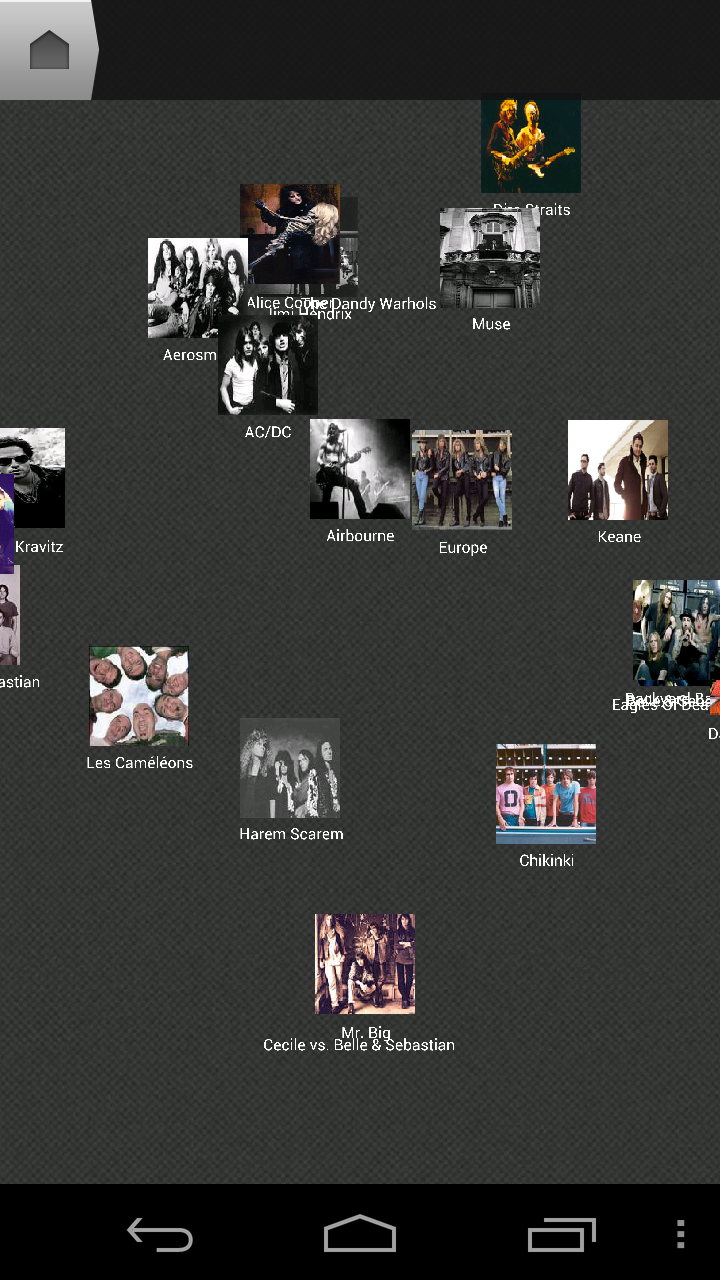
\includegraphics[width=0.4\textwidth]{figures/screen_mds_5_after_all_restnode_additions}
  \caption{Graph state after placements of all nodes outside the initial subset}
  \label{fig:screen_mds_5_after_all_restnode_additions}
\end{figure}

\newpage
\subsection{After 5 Placement Correction Iterations (MDS)}

Similar to the beginning of the calculations (depicted in Section ~\ref{subsec:mds-after-five-subset-iterations}), the spring model algorithm is again applied to the graph, but on all nodes at once. The previously approximated positions for many of the nodes have to be corrected (i.e., system stress has to be reduced) for the produced layout to increase significance. Some or many of the nodes are even at the wrong side of the graph, judging by the forces enacted by all other nodes. Application of a limited number of spring model iterations has the potential to improve the expressiveness of the layout greatly. Figure ~\ref{fig:screen_mds_6_after_5_cleanup_iterations} displays graph state after five spring model iterations.

\begin{figure}[H]
  \centering
    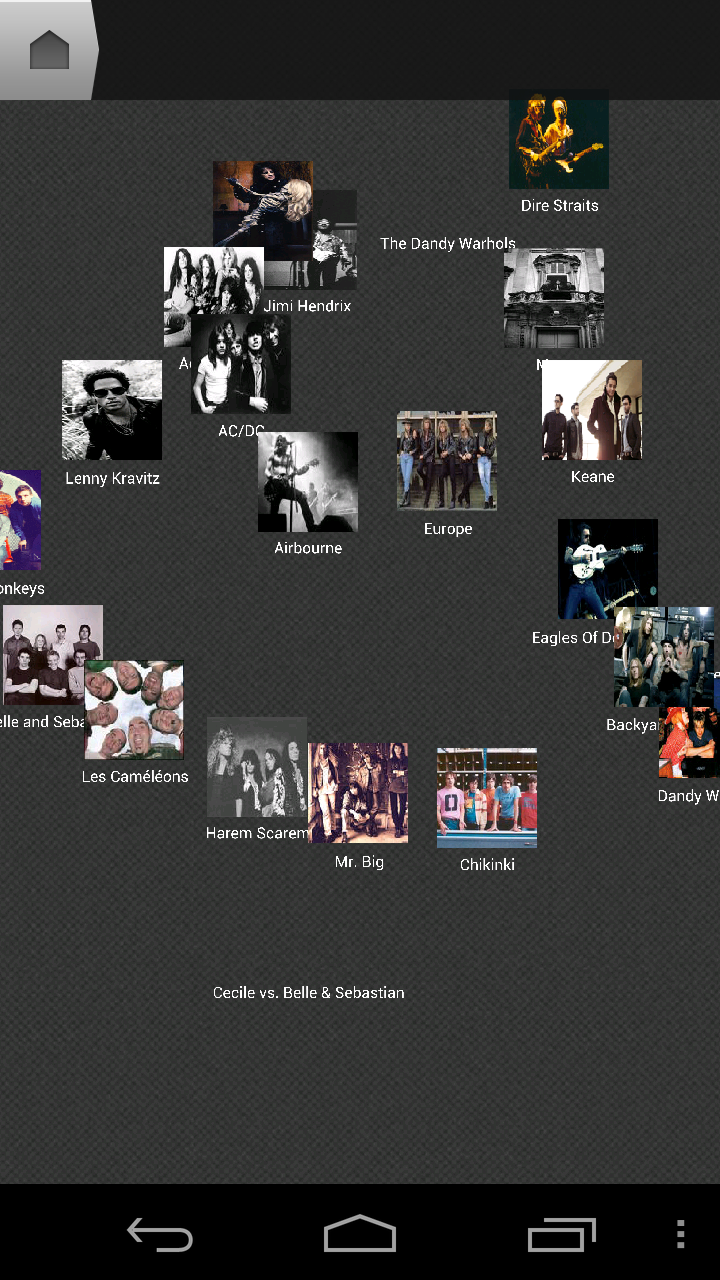
\includegraphics[width=0.4\textwidth]{figures/screen_mds_6_after_5_cleanup_iterations}
  \caption{Graph state after 5 spring model iterations of all nodes}
  \label{fig:screen_mds_6_after_5_cleanup_iterations}
\end{figure}

\newpage
\subsection{After 10 Placement Correction Iterations (MDS)}
\label{subsec:mds-after-ten-placement-iterations}

After 10 spring model iterations, the resulting layout is supposed to sufficiently satisfy the graph's similarity forces. The result is shown in figure ~\ref{fig:screen_mds_7_after_10_cleanup_iterations}, which also resembles the final outcome of the MDS algorithm. 
The graph's nodes have been laid out such that their centers' positions reduce system stress - not giving any heed to overlappings. Therefore, the process does not end here, but these overlappings have to be eliminated.

\begin{figure}[H]
  \centering
    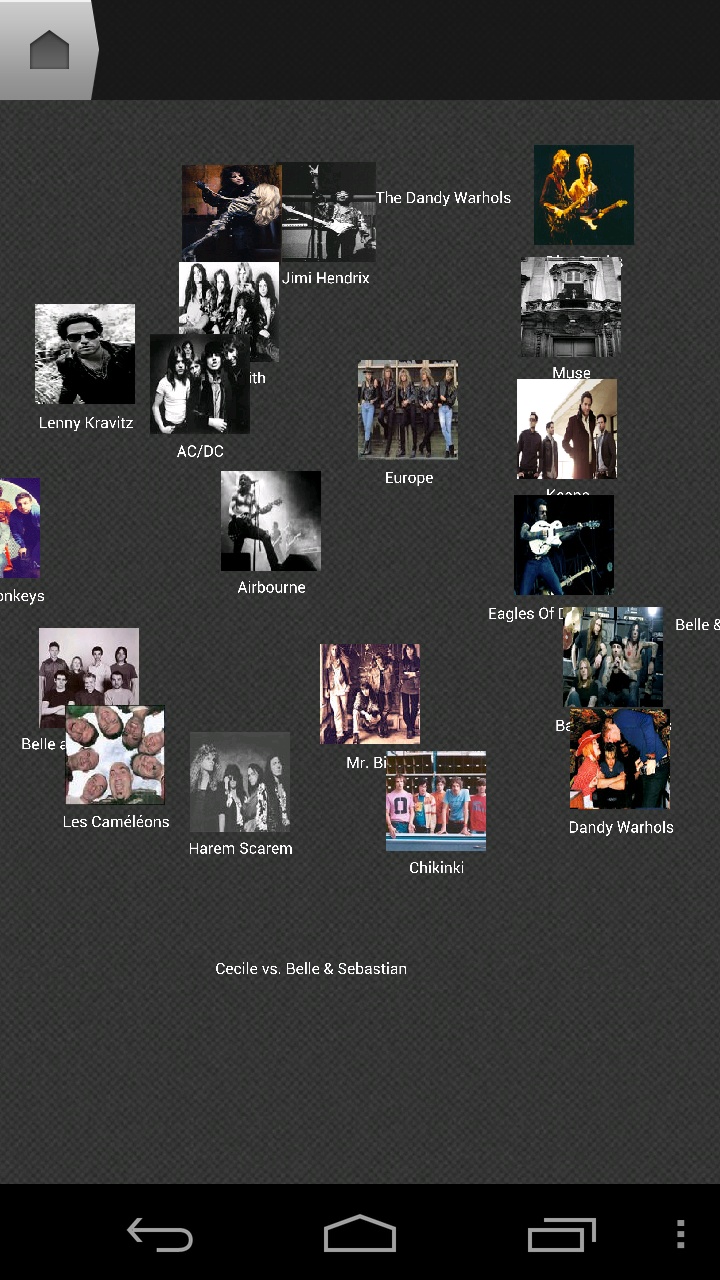
\includegraphics[width=0.4\textwidth]{figures/screen_mds_7_after_10_cleanup_iterations}
  \caption{Graph state after 10 spring force iterations of all nodes}
  \label{fig:screen_mds_7_after_10_cleanup_iterations}
\end{figure}

\newpage
\subsection{After Removal of Node Overlappings from 5 Nodes}

By applying the anti-overlap algorithm described in Section ~\ref{sec:removal-node-overlapping}, overlapping artist nodes are separated from each other. Figure ~\ref{fig:screen_mds_8_after_5_uncollided_nodes} shows the graph's state after five nodes have been processed, i.e. they have been repositioned such that they keep a certain margin to any other nodes.

\begin{figure}[H]
  \centering
    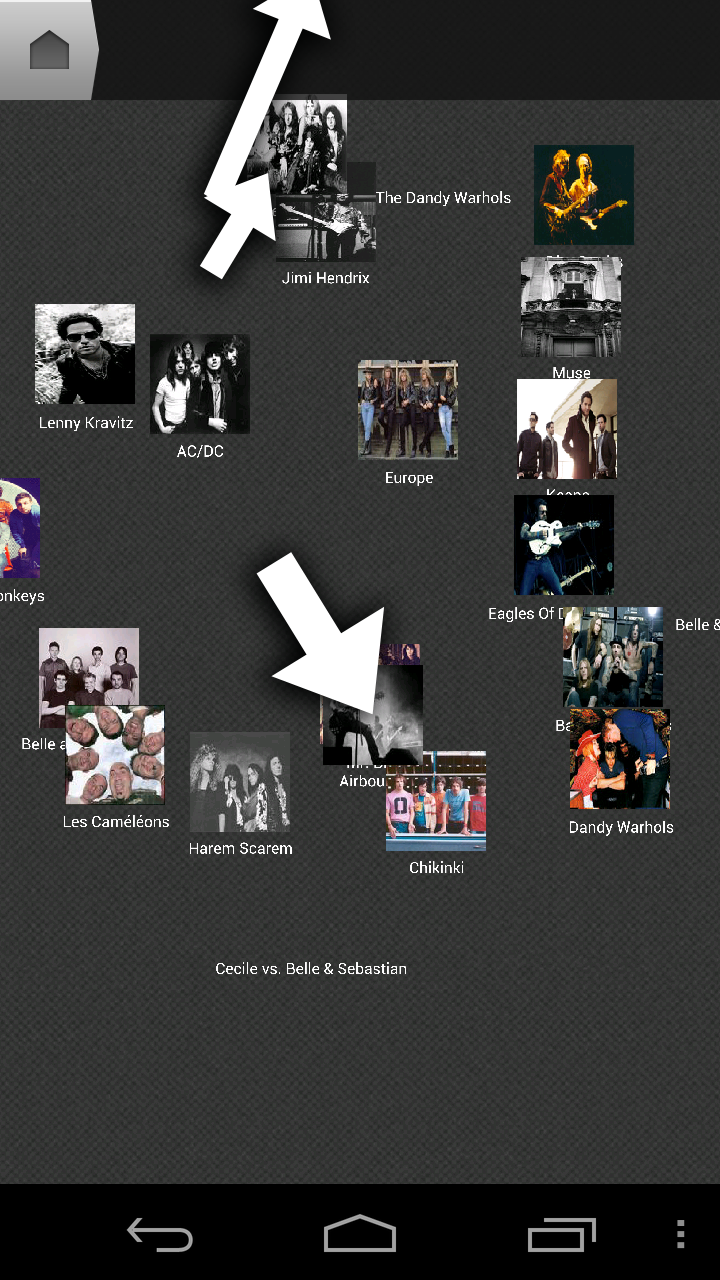
\includegraphics[width=0.4\textwidth]{figures/screen_mds_8_after_5_uncollided_nodes}
  \caption{Graph state after removal of node overlappings from 5 nodes}
  \label{fig:screen_mds_8_after_5_uncollided_nodes}
\end{figure}

\newpage
\subsection{After Removal of Node Overlappings from Half of All Nodes}

As a continuation of the last screenshot, the following figure ~\ref{fig:screen_mds_9_after_half_uncollided_nodes} depicts the graph's state after half of all artist nodes have been repositioned to avoid overlappings.

\begin{figure}[H]
  \centering
    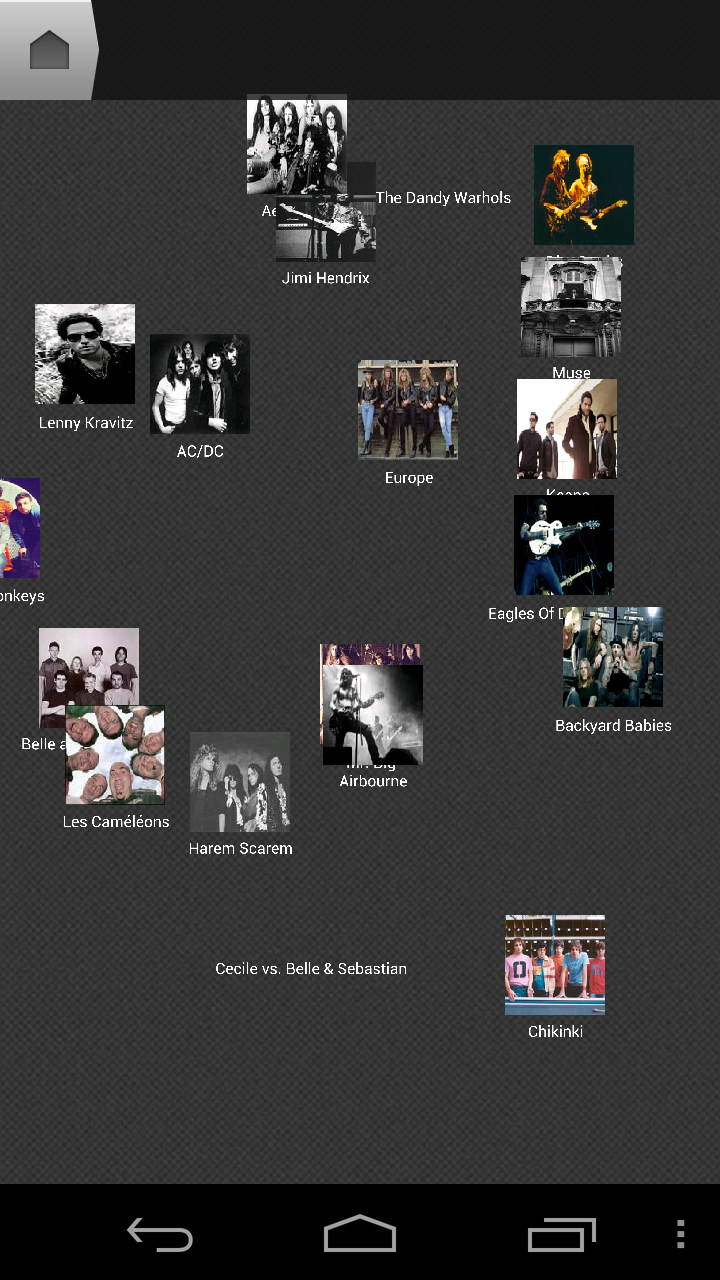
\includegraphics[width=0.4\textwidth]{figures/screen_mds_9_after_half_uncollided_nodes}
  \caption{Graph state after removal of node overlappings from half of all nodes}
  \label{fig:screen_mds_9_after_half_uncollided_nodes}
\end{figure}

\newpage
\subsection{After Removal of Node Overlappings from All Nodes}

Screenshot ~\ref{fig:screen_mds_10_after_all_uncollided_nodes} shows the final state of the graph, at the end of all computations. This is a compromise between the intermediate result shown in subSection ~\ref{subsec:mds-after-ten-placement-iterations}, and a user-friendly (easy to grasp) representation of the graph. Clearly, system stress has been increased by removal of node overlappings; but, the process has made the MDS algorithm's results readable and easily understandable. The resulting margin between the nodes is subject to adjustable parameters, leaving room for further optimization.

In the actual App implementation, this is the first state displayed to the user - all previous states are hidden from her. Subsequently, the App reacts to touch gestures in order to enable navigation and exploration of the structure on small screens (it's understood that screenshot~\ref{fig:screen_mds_10_after_all_uncollided_nodes} does not show all artists of the graph).

\begin{figure}[H]
  \centering
    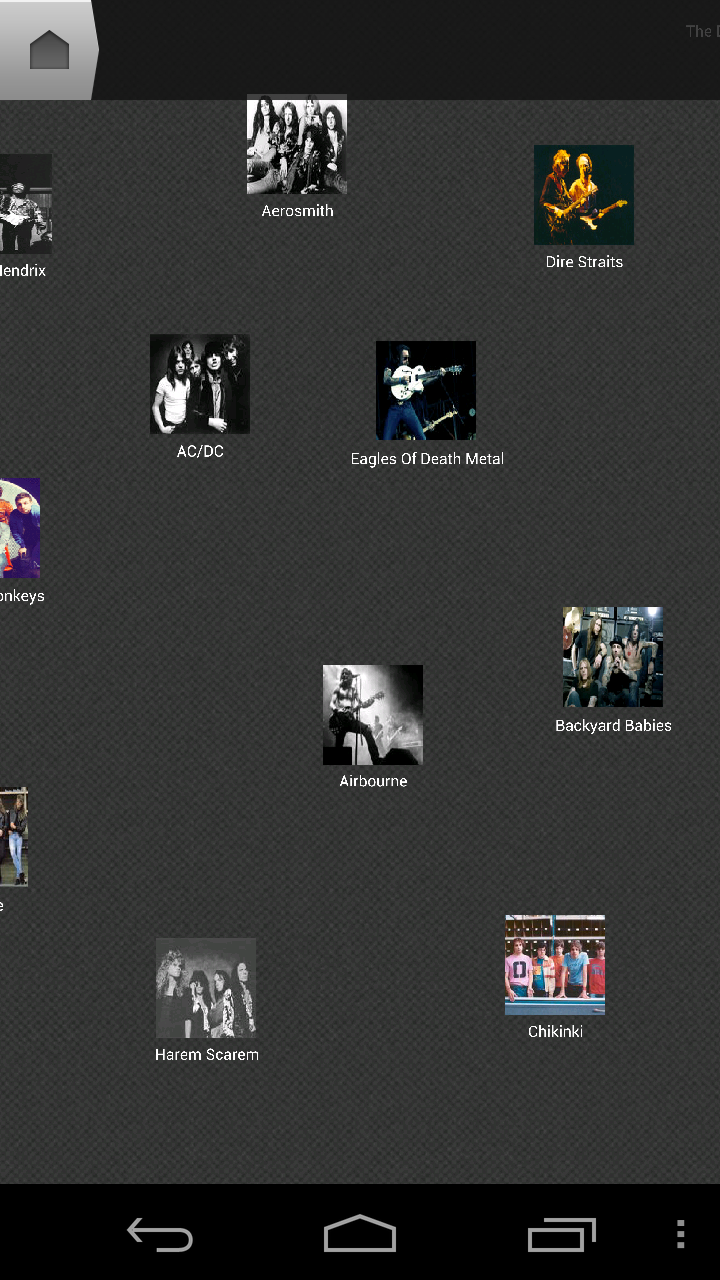
\includegraphics[width=0.4\textwidth]{figures/screen_mds_10_after_all_uncollided_nodes}
  \caption{Graph state after removal of node overlappings from all nodes}
  \label{fig:screen_mds_10_after_all_uncollided_nodes}
\end{figure}

\section{Retrieval of Music Metadata}

\subsection{Querying of Music Metadata on the Device}

Android has a cursor-based query system for multimedia metadata (kept up-to-date transparently by the
operation system). Creation of a cursor for all artists on the device is performed by program code like this:

\begin{verbatim}
Cursor artistCursor = mContext.getContentResolver().query(
	MediaStore.Audio.Artists.EXTERNAL_CONTENT_URI,
    artistProjection, null, null, null);
\end{verbatim}

Since the returned metadata also contains a unique key for each multimedia file, metadata can be
persisted in a database and later be reused without obstacles.
Metadata records themselves contain as much data as the user or the file-generating utility has defined
before the file was copied onto the device - clearly, files may not have any metadata available at all.

In the implementation of the App, such a cursor is traversed over all available music titles, and several entities are derived:

\begin{itemize}
	\item Artist,
	\item Album, and
	\item Track title.
\end{itemize}

While these entities are created, the implementation checks whether they already exist, and skips creation accordingly. Retrieved data is then stored in the App's on-device database.

\subsection{Retrieval of Music Metadata from Web Sources}

Last.fm \cite{url:lastfm} and Echonest \cite{url:echonest} are the de facto standards for music metadata retrieval in the world wide web, 
at the time of writing of this paper. The author has chosen to use both of these services for retrieval 
of semantic metadata for the implementation. 

After the device's music titles and their metadata have been retrieved, their metadata has to be augmented or corrected with the normalized data from external sources - Last.fm and Echonest. To ensure a stable mapping from on-device to remote music metadata records, these are fetched up front. For every artist, album, and track the App has retrieved from the device, a match is searched for in web sources. Search for matches is performed by sending an ordinary search query to the web sources, and metadata records are returned as a result. Excerpts of the acquired records are then stored in the App's on-device database.

\section{Retrieval of Similarity Data}

Ideally, the retrieval of similarities between artists should provide an exhaustive list of similarities between any two artists. But, as a real-world implementation must make do with actuality, workarounds had to be found which provide approximations to artist similarities.
Echonest's artist similarity results contain no similarity metric, but only the implicit ranking of artists. Therefore, the author of this thesis decided \textbf{not to use Echonest's similarity metrics}.

Last.fm's artist similarity data is, in contrast to Echonest, augmented with accurate similarity measures in the range of $[0 .. 1]$. But, it is not possible to query Last.fm for a certain similarity relationship between two certain artists - instead, the top 100 similar artists for a certain artist can be retrieved. It's clear that this way, many artist-to-artist relations in a music collection will not receive a similarity measure. Instead, a dedicated algorithm has to approximate similarity values which were not provided by Last.fm.

As Last.fm provides similarity value lists per artist ("'subject"'), it can be assumed that every relation to an artist not on the list has a similarity value within the interval \emph{[0 .. x], x = lowest known similarity of "'subject"' to any other artist}. Not having any more details at hand than this fact, the expected value of such an unknown similarity value is $x / 2$ - the author of this thesis decided to use this value as an approximation. In algorithm listing ~\ref{alg:similarity-approximation}, the algorithm to interpolate similarity values (which is being used in the App's implementation) is described. 

\begin{algorithm}[ht]
\SetKwData{SimilarArtists}{similarArtists}
\SetKwData{LowestMatch}{lowestMatch}
\SetKwData{ArtistOnDevice}{artistOnDevice}
\SetKwData{InnerArtistOnDevice}{innerArtistOnDevice}
\SetKwData{SimilarArtist}{similarArtist}
\SetKwData{ArtistSimilarity}{artistSimilarity}
\SetKwData{AllArtistSimilarities}{allArtistSimilarities}
\SetKwFunction{SizeOf}{sizeof}
\SetKwFunction{GetSimilarArtists}{getSimilarArtists}
\SetKwFunction{GetSimilarityMatch}{getSimilarityMatch}
\SetKwFunction{MakeArtistSimilarity}{makeArtistSimilarity}
\SetKwFunction{Matches}{matches}
\SetKwFunction{Put}{put}
\SetKwInOut{Input}{input}
\SetKwInOut{Output}{output}

\Input{List of all artists' metadata stored on the device}
\Output{List of similarities between each artist}

\BlankLine

\For{\ArtistOnDevice$\leftarrow$ firstArtist \KwTo lastArtist}{
  \SimilarArtists$\leftarrow$ \GetSimilarArtists(\ArtistOnDevice)\;
  \For{\InnerArtistOnDevice$\leftarrow$ firstArtist \KwTo lastArtist}{
    \If{\SizeOf{\SimilarArtists} $==$ 0}{\LowestMatch$\leftarrow$ 0\;}
    \Else{\LowestMatch$\leftarrow$ float-max-value\;}

    \For{\SimilarArtist$\leftarrow$ \SimilarArtists$.first$ \KwTo \SimilarArtists$.last$}{
      \If{\GetSimilarityMatch{\SimilarArtist} $<$ \LowestMatch}
         {\LowestMatch$\leftarrow$ \GetSimilarityMatch{\SimilarArtist}\;}
      \If{\Matches{\SimilarArtist, \InnerArtistOnDevice}}
        {\ArtistSimilarity$\leftarrow$ \MakeArtistSimilarity{\ArtistOnDevice, 
          \InnerArtistOnDevice, \GetSimilarityMatch{\SimilarArtist}}\;
        \textbf{break}\;
	  }
    }

	\If{\SizeOf{\SimilarArtists} $==$ 0}{\ArtistSimilarity$\leftarrow$ \MakeArtistSimilarity{\ArtistOnDevice, 
      \InnerArtistOnDevice, 0}\;}
    \ElseIf{\ArtistSimilarity $==$ 0}{\ArtistSimilarity$\leftarrow$ \MakeArtistSimilarity{\ArtistOnDevice, 
      \InnerArtistOnDevice, \LowestMatch $/ 2$}\;}

	\Put{\AllArtistSimilarities, \ArtistSimilarity}\;
  }
}
\Return \AllArtistSimilarities\;
\BlankLine
\caption{Similarity Approximation Algorithm}\label{alg:similarity-approximation}
\end{algorithm}

\section{Implementation of Multidimensional Scaling}
\label{subch:implementation-mds}

The selected MDS algorithm has already been discussed broadly in Chapter ~\ref{ch:computation}. Implementation of this algorithm required the creation of a number of helper and data classes, but on the whole, the implementation follows the pseudocode from Chapter ~\ref{ch:computation} closely. To better illustrate step 3. from the mentioned pseudocode, the implementation part is included in the algorithm listing ~\ref{alg:nearest-neighbor-positioning}.

\begin{algorithm}[ht]
\SetKwData{Subject}{subject}
\SetKwData{NearestNode}{nearestNode}
\SetKwData{CurrentSubsetNodes}{currentSubsetNodes}
\SetKwData{DistanceToNearestNode}{distanceToNN}
\SetKwData{UpperRightQuadrant}{urQuadrant}
\SetKwData{LowerRightQuadrant}{lrQuadrant}
\SetKwData{UpperLeftQuadrant}{ulQuadrant}
\SetKwData{LowerLeftQuadrant}{llQuadrant}
\SetKwData{UpperRightStress}{urStress}
\SetKwData{LowerRightStress}{lrStress}
\SetKwData{UpperLeftStress}{ulStress}
\SetKwData{LowerLeftStress}{llStress}
\SetKwData{CurrentSubsetNode}{currentSubsetNode}
\SetKwData{MinStress}{minStress}
\SetKwData{SumOfForcesOnSubject}{sumOfForcesOnSubject}
\SetKwData{InitialSubset}{initialSubset}
\SetKwFunction{Add}{add}
\SetKwFunction{GetNearestNode}{getNearestNode}
\SetKwFunction{GetDistanceBetween}{getDistanceBetween}
\SetKwFunction{GetPointInQuadrant}{getPointInQuadrant}
\SetKwFunction{GetStress}{getStress}
\SetKwFunction{Min}{min}
\SetKwFunction{SetPosition}{setPosition}
\SetKwFunction{MakeVector}{makeVector}
\SetKwFunction{Force}{force}
\SetKwFunction{Displace}{displace}
\SetKwInOut{Input}{input}
\SetKwInOut{Output}{output}


\Input{Subject [the node to be positioned near any other node]}
\Input{InitialSubset [the initial nodes subset]}
\Input{CurrentSubsetNodes [the nodes subset incrementally populated]}
\Output{No return value; Subject node has been optimally positioned}

\BlankLine

\NearestNode$\leftarrow$ \GetNearestNode{\Subject, \CurrentSubsetNodes}\;
\DistanceToNearestNode$\leftarrow$ \GetDistanceBetween{\Subject, \NearestNode} $*$ DISTANCE-CONSTANT\;

\UpperRightQuadrant$\leftarrow$ \GetPointInQuadrant{1, 1, \DistanceToNearestNode, \NearestNode}\;
\LowerRightQuadrant$\leftarrow$ \GetPointInQuadrant{1, -1, \DistanceToNearestNode, \NearestNode}\;
\UpperLeftQuadrant$\leftarrow$ \GetPointInQuadrant{-1, 1, \DistanceToNearestNode, \NearestNode}\;
\LowerLeftQuadrant$\leftarrow$ \GetPointInQuadrant{-1, -1, \DistanceToNearestNode, \NearestNode}\;

\tcc{Calculate Stress for upper \& lower, right \& left quadrants...}

\MinStress$\leftarrow$ \Min{\UpperRightStress, \LowerRightStress, \UpperLeftStress, \LowerLeftStress}\;

\If{\UpperRightStress $==$ \MinStress}{\SetPosition{\Subject, \UpperRightQuadrant}\;}
\ElseIf{\LowerRightStress $==$ \MinStress}{\SetPosition{\Subject, \LowerRightQuadrant}\;}
\ElseIf{\UpperLeftStress $==$ \MinStress}{\SetPosition{\Subject, \UpperLeftQuadrant}\;}
\Else{\SetPosition{\Subject, \LowerLeftQuadrant}\;}

\For{i$\leftarrow$ 1 \KwTo QUADRANT-REFINING-ITERATIONS}{
  \SumOfForcesOnSubject $\leftarrow$ \MakeVector\;
  \For{$node\leftarrow$ \InitialSubset$.first$ \KwTo \InitialSubset$.last$}{
     \Add{\SumOfForcesOnSubject, \Force{\Subject, $node$}}\;
  }
  \Displace{\Subject, \SumOfForcesOnSubject}\;
}

\BlankLine
\caption{Nearest-Neighbor Positioning Algorithm}
\label{alg:nearest-neighbor-positioning}
\end{algorithm}

\section{Implementation of Removal of Node Overlappings}
\label{subch:implementation-overlapping}

The algorithm used for the removal of node overlappings has been shown in Section ~\ref{ch:visualization}. The actual implementation required some pragmatic changes, therefore the code is listed in the algorithm listing ~\ref{alg:removal-node-overlappings}.

\begin{algorithm}[ht]
\SetKwData{Subject}{subject}
\SetKwData{SubjectDisplacementVector}{subjectDisplacementVector}
\SetKwData{NodeCentersDistance}{nodeCentersDistance}
\SetKwData{CollisionCandidate}{collisionCandidate}
\SetKwData{RandomMargin}{randomMargin}
\SetKwData{NodesWithoutOverlap}{nodesWithoutOverlap}
\SetKwFunction{Randomize}{randomize}
\SetKwFunction{GetEuclideanDistance}{getEuclideanDistance}
\SetKwFunction{MakeVector}{makeVector}
\SetKwFunction{SetVectorLength}{setVectorLength}
\SetKwFunction{Displace}{displace}
\SetKwInOut{Input}{input}
\SetKwInOut{Output}{output}


\Input{Subject [node to be freed from overlappings with others]}
\Input{NodesWithoutOverlap [nodes to which this algorithm has been applied]}
\Output{No return value; Subject node has been freed of overlappings}

\BlankLine

  \For{i$\leftarrow$ 0 \KwTo ITERATIONS}{
    \For{\CollisionCandidate$\leftarrow$ \NodesWithoutOverlap$.first$ \KwTo \NodesWithoutOverlap$.last$}{
      \NodeCentersDistance$\leftarrow$ \GetEuclideanDistance{\Subject, \CollisionCandidate}\;
      \RandomMargin$\leftarrow$ \Randomize{}\;

\tcc{NODES-SIZE: diagonal through an artist's depiction square, the maximally needed displacement
	  to separate two overlapped artist nodes.}
	
      \If{\NodeCentersDistance $< NODES-SIZE +$ \RandomMargin}{
        \SubjectDisplacementVector$\leftarrow$ \MakeVector{\CollisionCandidate, \Subject}\;
		\SetVectorLength{\SubjectDisplacementVector, NODES-SIZE $-$ \NodeCentersDistance $+$ \Randomize{}}\;
        \Displace{\Subject, \SubjectDisplacementVector}\;
      }
    }
  }

\BlankLine
\caption{Removal of Node Overlappings Algorithm}
\label{alg:removal-node-overlappings}
\end{algorithm}


The optimized algorithm has a predefined number of iterations, by the end of which a node should no longer overlap any other nodes. This number has to be chosen carefully - too high and the overall computation duration will increase linearly, too low and not all node overlappings will be removed.

\section{Visualization Details}

Apart from the previously described computational algorithms, the App features a number of components or behavior not contained in the Android operating system. In the following, the most interesting features aiding the visualization of content will be described.

\subsection{Drawing with OpenGL}

Android provides App developers with the possibility to implement three-dimensional viewports in OpenGL ES \cite{url:opengles}, which is a downsized version of ordinary OpenGL and meant for implementation in handheld devices. OpenGL is a specification which is used as a blueprint by operating systems vendors and GPU producers alike. An OpenGL context can be seen as a state-machine which is manipulated by external API calls.

While the prototype shall implement a 2D visualization, its implementation in OpenGL (which is a 3D drawing specification) is necessary to provide a reasonably high framerate. Early prototype tests with a strict 2D implementation (Android 2D canvas drawing) showed that image rendering let the framerate drop considerably, so that viewport zooming, panning, and animations were no longer smooth to the human eye. The app's usability suffered from this, and so the prototype was rebuilt using OpenGL. The reason why OpenGL performs better in this context is that GPUs are better suited for handling images (textures) than CPUs, because their architecture and instruction sets are primarily dedicated to rendering.

In order to be able to employ OpenGL for graph rendering, the author of this thesis had to create a number of abstract meta classes and find a way to resemble user interactions in the drawn 3D picture. As mentioned before, the objective was to draw pseudo-2D, such that all music objects are displayed as pictures, viewed from the top. Accordingly, the viewport has to move sideways when the user moves one finger over the touchscreen, and it has to change its distance to the graph objects when the user zooms.

\subsection{Touchscreen Handling}

With the advent of smartphones, strong conventions have been established by phone vendors which determine how users may interact with the smartphone. Touchscreen technology provides a more immediate way of interaction than previous systems, allowing users to seemingly interact with the very objects they want to manipulate (as opposed to moving views and cursors with hardware buttons).
There are three touchscreen gestures supported by the App's implementation:

\begin{itemize}
	\item \textbf{Panning/Scrolling} - The user taps the finger onto the screen surface, does not let 
	go, and pulls the finger across the surface. As long as the finger does not part from the surface, 
	the "'pan/scroll"' is active.
	\item \textbf{Zooming} - The user rests two fingers on the screen surface, and changes the distance
	between her finger tips. If the distance decreases, then the zoom factor will increase; and vice versa.
	Ideally, the touched points would always stay right under the user's finger tips, but in the built
	App prototype, this has not been achieved, because of the three-dimensional nature of the OpenGL
	rendering process.
	\item \textbf{Tapping} - The user taps her finger onto the screen surface at a point on which the
	desired object is located, and lets go again immediately. The App then reacts to this interaction
	with an adequate response or action, depending on the current state of the user interface.
\end{itemize}

\subsection{Animations}

To make transitions between view states in the App smoother and easier to follow for users, animations have been implemented to do so. It has been shown in an empirical study that comprehension of changes can be improved by adding animations ~\cite{Schlienger:2007}.

\textbf{Whole-screen transition} - If the user chooses to display an artist's albums, the transition to the next Activity (fullscreen Android layout component) is implemented as a fade-over animation, meaning that the second screen is added as an overlay and its alpha channel is animated from 0 to 1. This way, the user is able to notice the change of context without being disturbed by untraceable changes.

\textbf{Artist Node animation} - If the user selects an artist by tapping, the artist's image depiction is moved on the z-axis towards the virtual camera - appearing nearer to the viewport. This puts an emphasis on the selected artist and makes for a pleasing optical effect. As OpenGL is a low-level framework, animations like this have to be implemented by the developer - keeping track of animation start and projected end time, and determining the state for every newly drawn frame.

\textbf{Context-related graph area darkening} - If the user chooses to display an artist's related (similar) artists, the graph area darkens over all other currently displayed artists, to put an emphasis on the selected artist and its related artists. This effect is achieving by adding a rectangle between the emphasized artists and the others, which is at first transparent and then gains opacity through an animation.

\section{Structure of the App}

The prototypical App implementation is targeted at the Android operating system. In this section, some implementation specifics will be given for better reproducability.

\subsection{Activities}

The App's UI stack consists of two Activities (screens):

\begin{itemize}
	\item \textbf{Loading Activity} - Fetching metadata from the internal storage and web sources, and compilation of the same is a lengthy process, and therefore a dedicated Activity exists in the App, displaying progress indicators.
	\item \textbf{Artists Activity} - The main screen of the App, showing all artists in the user's music collection, laid out such that nearness between artists implicates similarity.
	\item \textbf{Albums Activity} - The secondary screen, displaying an artist the user has selected on the previous screen, along with their albums.
\end{itemize}

\subsection{Classes and Packages}

In the following, figures of the App's class and package structure will be depicted. The reader can refer to their descriptions in the figures' captions.

\begin{figure}[H]
  \centering
    \fbox{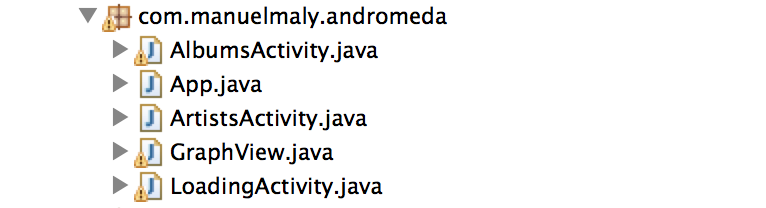
\includegraphics[width=0.7\textwidth]{figures/package-main}}
  \caption{The App's main package, containing Activities, the root App class (a singleton in Android), and a generic graph view class.}
  \label{fig:package-main}
\end{figure}

\begin{figure}[H]
  \centering
    \fbox{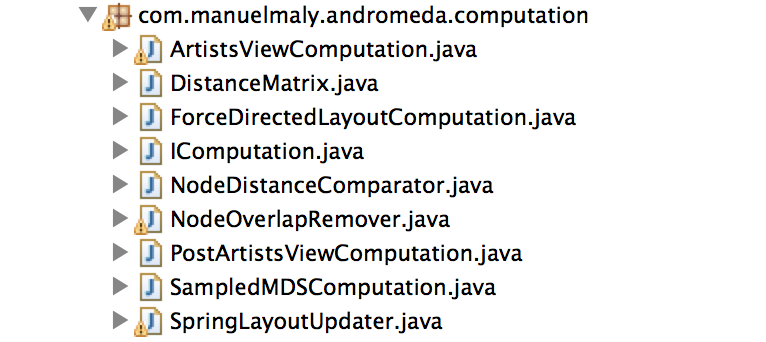
\includegraphics[width=0.7\textwidth]{figures/package-computation}}
  \caption{Package containing all classes and interfaces related to computation - MDS layout, spring layout, node overlap removal, and intermediate helper computations.}
  \label{fig:package-computation}
\end{figure}

\begin{figure}[H]
  \centering
    \fbox{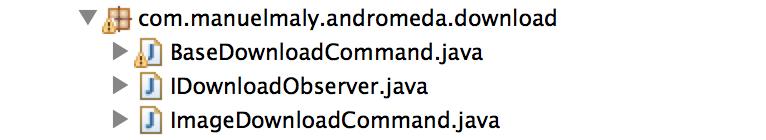
\includegraphics[width=0.7\textwidth]{figures/package-download}}
  \caption{Classes related to download of content, like images.}
  \label{fig:package-download}
\end{figure}

\begin{figure}[H]
  \centering
    \fbox{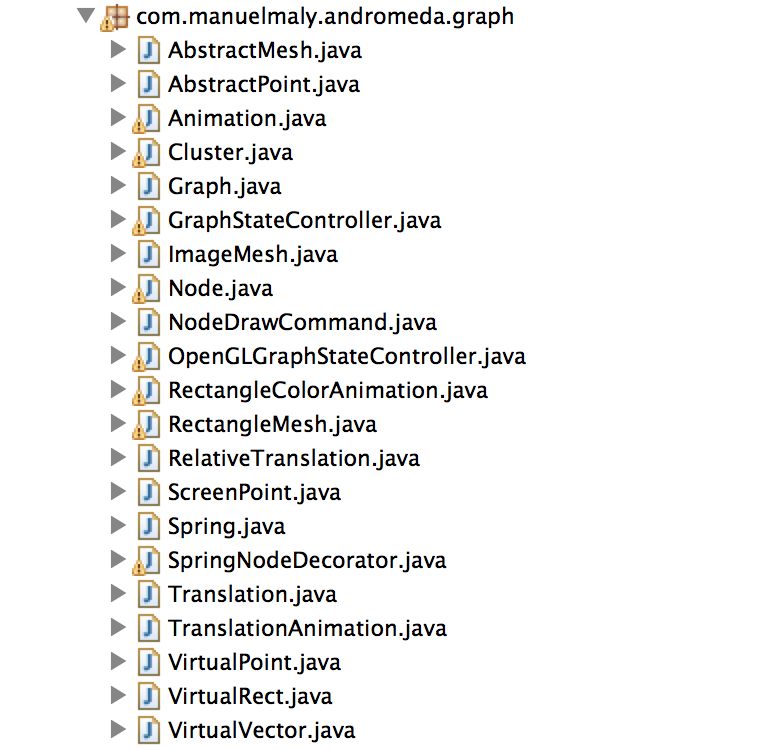
\includegraphics[width=0.7\textwidth]{figures/package-graph}}
  \caption{Graph-related and auxiliary classes, with their functionality ranging from graph nodes and graph state retention to animation state helpers.}
  \label{fig:package-graph}
\end{figure}

\begin{figure}[H]
  \centering
    \fbox{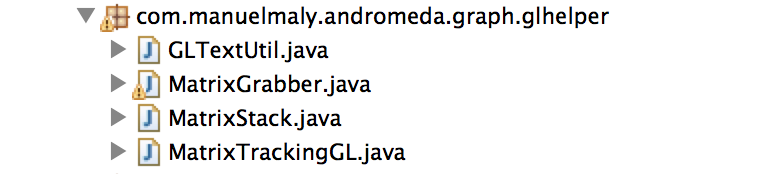
\includegraphics[width=0.7\textwidth]{figures/package-glhelper}}
  \caption{Package containing OpenGL helper classes, as needed for the use of OpenGL ES in Android.}
  \label{fig:package-glhelper}
\end{figure}

\begin{figure}[H]
  \centering
    \fbox{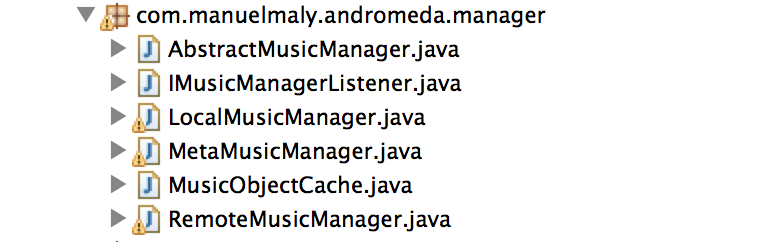
\includegraphics[width=0.7\textwidth]{figures/package-manager}}
  \caption{Management classes responsible for querying and storing music metadata on the device and on web sources.}
  \label{fig:package-manager}
\end{figure}

\begin{figure}[H]
  \centering
    \fbox{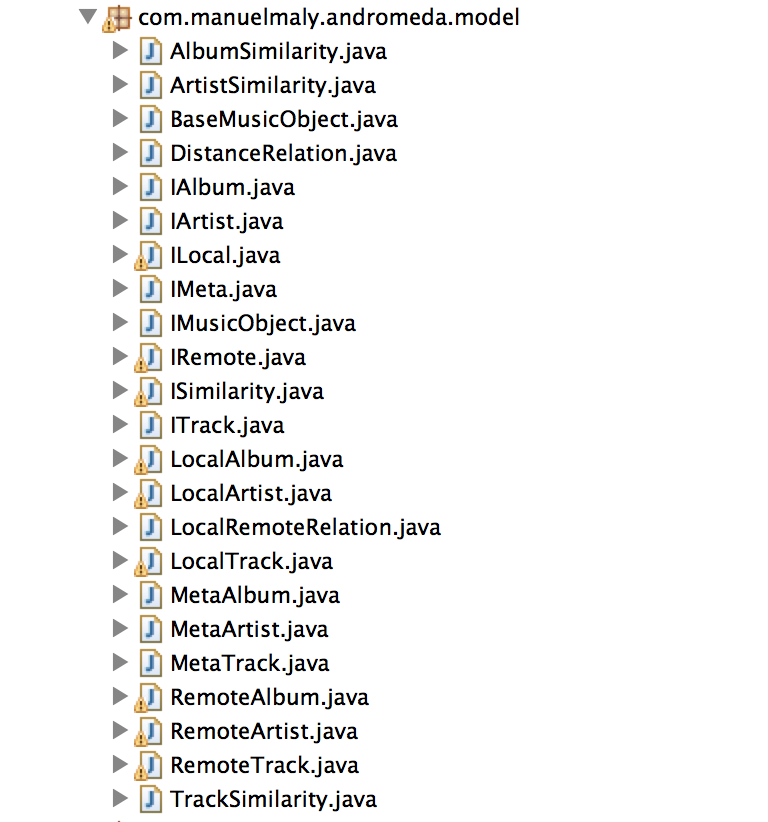
\includegraphics[width=0.7\textwidth]{figures/package-model}}
  \caption{Package with model classes which hold music metadata from both the device and web sources.}
  \label{fig:package-model}
\end{figure}

\begin{figure}[H]
  \centering
    \fbox{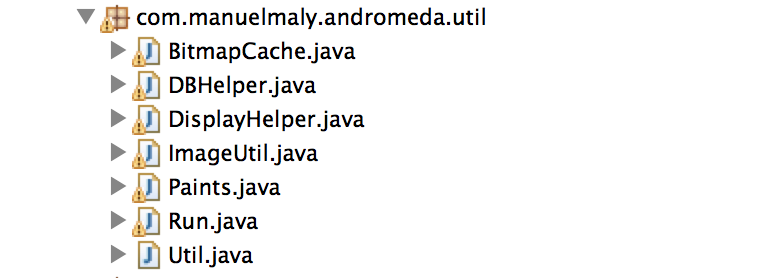
\includegraphics[width=0.7\textwidth]{figures/package-util}}
  \caption{Utility components which provide functionality to the rest of the App's classes, most of them being generic and exchangeable.}
  \label{fig:package-util}
\end{figure}

\begin{figure}[H]
  \centering
    \fbox{
\includegraphics[width=0.7\textwidth]{figures/package-widget}}
  \caption{Package containing widget classes which could be used in most Android apps - currently containing only one such component.}
  \label{fig:package-widget}
\end{figure}

\subsection{Third Party Libraries}

\begin{itemize}
	
	\item \textbf{jEn-api}, an Echonest API library for Java, also working in Android apps. \\
License: \emph{New BSD License}

	\item \textbf{lastfm-java}, an unofficial Last.fm API library for Java, also working in Android apps. \\
License: \emph{New BSD License}

	\item \textbf{ORMLite}, a low-profile object relational mapper for SQLite in Java, also working in Android apps. \\
License: \emph{ISC License}

	\item \textbf{JSON.simple}, a JSON (JavaScript Object Notation) parser for Java, also working in Android apps. \\
License: \emph{Apache 2.0 License}

	\item \textbf{Android Support Library v4}, a library provided by Google to enable more recent Android features for older OS versions. \\
License: \emph{Apache 2.0 License}

	\item \textbf{Android Annotations}, a compile-time library which generates code from Java annotations, to allow pseudo-dependency injection and more advanced features. \\
License: \emph{Apache 2.0 License}

\end{itemize}

\section{Summary of this Section}

This chapter has explained the components, algorithms, and concepts used to construct a prototype demonstrating the visualization of artist similarity, runnable on mobile Android devices.

Algorithms and the flow of information between them has been described, both for the visualization of a music library (on-device metadata extraction, matching, web source metadata extraction and interpolation, layout generation, removal of node overlappings, display of the graph to the user), and for artist discovery (querying of related artists from web sources, their integration into the layout, and continuous rearrangement via a force-based layout algorithm).
Thereafter, different states of the App prototype while executing the previously described algorithms have been illustrated, using screenshots.

Retrieval of music metadata from the user's device and web sources, and retrieval of similarity data from web sources has been described in detail. Since this similarity data may be incomplete, an interpolation algorithm for unknown values has been given.
A part of the MDS algorithm (already described in length in Chapter ~\ref{ch:computation}), the  positioning of graph nodes based on system stress minimization, has been detailed as pseudocode. The algorithm for the removal of node overlappings in the graph was also shown.
To provide some details about visualization and the App's user interaction model, OpenGL drawing, touchscreen gestures, and animations were elaborated on.

Finally, a short introduction to the Android operating system was given, and the prototype App's structure (Activities and other classes) and third party libraries were detailed.
In order to evaluate how the prototype ("'Andromeda"') described in the previous chapter performs when compared to other music library visualizations, a user study has been carried out and analyzed. As the publicly available mobile apps for Android don't support any form of artist discovery, the scope of the user study will be limited to the visualization of artists, and the impact of using Andromeda on usage metrics, as opposed to using other predetermined music apps (visualization methods).

In this chapter, the conception, execution, and analysis of the user study will be described, in this order:

\begin{itemize}
	\item \textbf {Hypotheses} - Defines a list of 5 hypotheses to be examined by the user study.
	\item \textbf {Metrics and Tools} - Describes how the study will gather which data.
	\item \textbf {Population, Setup, and Process} - Lists execution details of the study, together with a description of the test participants.
	\item \textbf {Results and Data} - Summarizes the gathered data and provides statistical key figures.
	\item \textbf {Analysis and Discussion} - Gives a discussion of the study's results and notes on the acceptance or rejection of previously defined hypotheses.
\end{itemize}

\section{Hypotheses}

As described in \cite{Christopher03thoughtson}, a user study for a visualization can be performed because of various reasons: 

\begin{enumerate}
	\item To show the practicality of a visualization,
	\item To find out why a visualization is effective, or
	\item To show that a theory from another domain applies to a visualization technique under practical conditions.
\end{enumerate}
	
Depending on which of these is the underlying motivation, a hypothesis can be established, to be verified by the user study. Obviously, a user study can not as definitely accept or dismiss a hypothesis as a double-blind experiment with a huge test sample (as used in other domains) can. This is due to various reasons - e.g., experiment variables cannot be controlled as tightly with the available budget, the context of testing a visualization does not lend itself to methods isolating individual test factors, and the context of this thesis does not allow for a large sample. Still, the study will give a hint towards or against acceptance of the hypothesis.

The hypotheses to be evaluated by the following user study are as follows:

\begin{itemize}
	\item H1: Andromeda Andromeda (both similarity-based and randomized layouts) allows forming of a more detailed mental model of the music collection than the other music apps under test, resulting in better memorization of the collection's artists.
	\item H2: Andromeda Andromeda (both similarity-based and randomized layouts) allows faster finding of certain artists by name than the other music apps.
	\item H3: Andromeda Andromeda (both similarity-based and randomized layouts) allows faster re-finding of certain artists by name after closing the app by name than the other music apps.
	\item H4: Andromeda Andromeda with similarity-based artist representation allows for faster finding of an artist with highest similarity to a predefined seed artist.
	\item H5: Andromeda Andromeda (both similarity-based and randomized layouts) allows faster finding of 3 artists by mood than the other music apps.
\end{itemize}

Apart from the verification of these hypotheses, the study will also use questionnaires to determine qualitative metrics commonly used in user interface studies. Those establish qualitative indicators on user satisfaction and general usability of Andromeda which do not support or decline the hypothesis, but might be of interest to the reader nonetheless.

\section{Metrics and Tools}

\subsection{Task-Based Evaluation of Multiple Visualizations}

In order to evaluate the visualization which is the center of this thesis, its performance is compared to other established methods in the mobile computing area. This comparison is established by letting test users perform predefined tasks with Andromeda and other, production-grade, music apps for Android. Several metrics are recorded during these tests which can be evaluated afterwards. The outcome of these recordings will give a hint on how well the visualization method (based on artist similarity) resonates with users, as compared to other methods.

The concrete visualizations which will be compared are:

\begin{itemize}
	\item Andromeda for Android (prototype built for this thesis)
	\item Modified Andromeda for Android, with a simple randomized layout instead of MDS using spring model as 2D projection algorithm
	\item "'Play Music"', the current Android system music player, also availabe on the Play Store \cite{url:playmusic}
	\item "'Jukefox"', a 3D music player app for Android available on the Play Store \cite{url:jukefox}
\end{itemize}

The modified version of Andromeda (with randomized layout) is expected to perform worse in the tests than the unmodified, original version of Andromeda. Both shall be tested in order to evaluate how much better the unmodified version with the 2D-projection using artist similarities performs compared to an app which has the same interface, but where randomized positions are assigned to each artist.

Their succession in the tests will be varied, to reduce learning effects carrying over into the study results. Side-by-side screenshots of all tested apps can be seen in Figure ~\ref{fig:apps_screenshots}.

It can not be avoided that some users are already familiar with production level apps. Concretely, two users had used the "'Play Music"' app before entering the test, as was reported by them during the tests. It is likely that this gave the "'Play Music"' app an advantage over the other apps - however, as will be shown later on, this app fared consistently very good in most of the tasks, and not only for these two users. The other production level app, "'Jukefox"', was not known to any test users prior to the tests.

\begin{figure}[H]
  \centering
    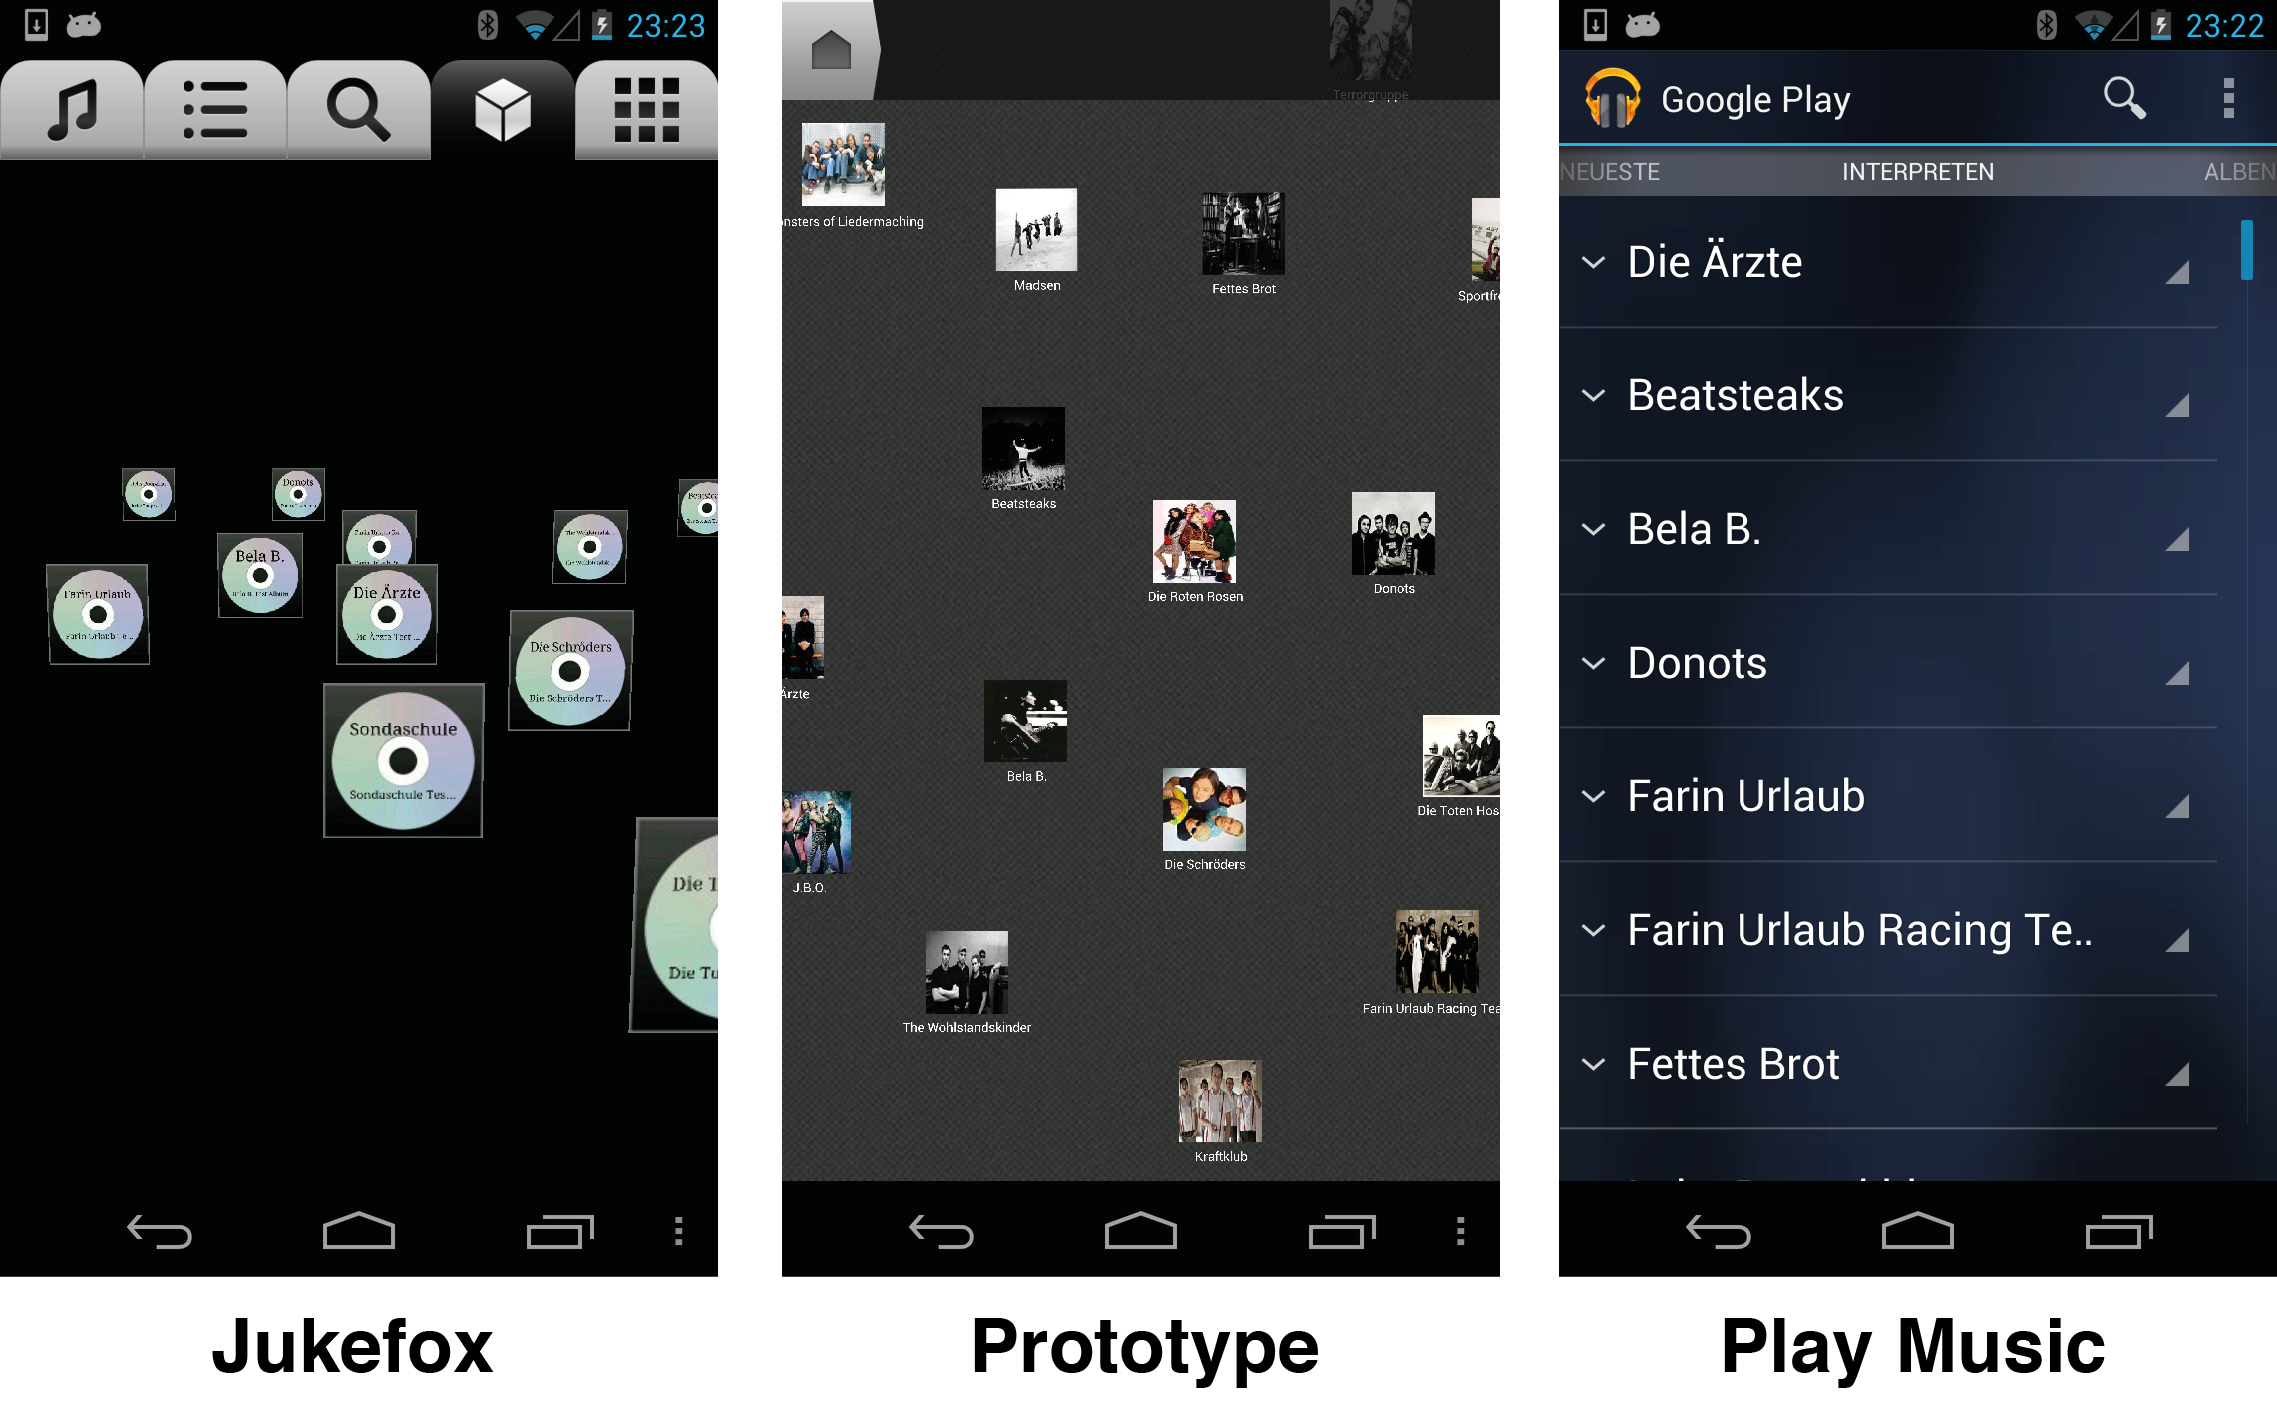
\includegraphics[width=1\textwidth]{figures/apps_screenshots}
  \caption{Screenshots of All Tested Apps}
  \label{fig:apps_screenshots}
\end{figure}

\subsection{AttrakDiff 2}

AttrakDiff 2 \cite{tubiblio21687} is a method to measure attractiveness of software to its users. It originates from the domain of user experience and is based on observations in psychology \cite{DBLP:journals/ijhci/Hassenzahl01}. AttrakDiff measures hedonic and pragmatic quality of a product, which assesses its luxurious or stimulating vs purely functional aspects. These qualities are important from a user perspective, as the perceived quality and functionality of a product can have an impact on how many users will use it for how often, or whether any people will use it at all.

Measuring the hedonic and pragmatic qualities of Andromeda will provide no isolatable statements about the usefulness of the abstract main topic of this thesis (visualization of artist similarity). But, it will give a hint of how well Andromeda resonates with users' usage patterns and aesthetic taste. The concrete questionnaire can be found in appendix ~\ref{app:attrakdiff}.

\subsection{System Usability Scale}

The System Usability Scale (SUS) has been introduced in 1986 and consists of 10 strong statements, to which a test person agrees or does not agree \cite{Lewis:2009}. Agreement or disagreement is expressed through a scale from 1 to 5. By subtraction of 1 and multiplication by 2,5, the maximum sum of all items is normalized to 100. The outcome of such an evaluation is a measure for the tested system's general usability.

Similar to AttrakDiff 2, this measure is not representative of the visualization method alone, but of Andromeda as a whole. The concrete questionnaire can be found in appendix ~\ref{app:sus}.

\subsection{Pre- and Post-Testing Questionnaires}

To find out about personal facts and opinions of the test users, questionnaires before and after the other evaluations ask for certain information. The Pre-Testing Questionnaire asks for general personal data, like age, profession, and self-assessments concerning usage of music software, while the Post-Testing Questionnaire asks for impressions of Andromeda. This data helps to put the test results into context, regarding the user demography and emotional attitude towards Andromeda. The concrete questionnaires can be found in appendices ~\ref{app:pretest} and ~\ref{app:posttest}.

\section{Population, Setup, and Process}

In the following, the setup and process of the user testing process will be described.

\begin{itemize}
  \item The study is performed with a sample of \textbf{10 test users}. 
  \item The testing takes place in a well-lit room with low noise level.
  \item Each testing takes place in one single session.
  \item Each testing consists of the following steps:
	\begin{itemize}
		\item Introduction by the tester
		\item Pre-Testing questionnaire is filled out by the test person
		\item Task-based evaluation is performed in a strict order, under close observation of the tester
		\item AttrakDiff 2 questionnaire is filled out by the test person	
		\item System Usability Scale questionnaire is filled out by the test person	
		\item Post-Testing questionnaire is filled out by the test person
	\end{itemize}
\end{itemize}

\subsection{Task-Based Evaluation Details}
\label{subsec:task-based-evaluation}

As mentioned previously, the comparison of visualization methods can be done by letting test users perform tasks, and compare how they interact with each visualization. 

This evaluation will make use of different music collections:

\begin{itemize}
	\item \textbf{One personalized collection for every user}, based on her favorite artist as a seed and all other artists being derived from a list of the most similar to the seed artist. Each test user's list was created by first asking the test user for her favorite artist (seed artist), then querying Last.fm for the 20 most similar artists of this seed artist, generating short music files (with meaningless bitstream content) with corresponding metadata, and storing the generated files in the device's media storage. The Android OS subsequently scanned the files and updated its internal music metadata caches, which are then used by all four apps under test. The rationale for this process is that this collection will likely contain mainly artists the user is familiar with, making it easier to form a mental model of the respective collection. The test tasks performed with these personalized music collections also depend on the user's rough knowledge of the contained artists (like selecting artists for a given mood).
	\item \textbf{Four predefined music collections} which contain artists which ideally are not known to the user (but knowledge of these artists has not been checked for the users, because this would skew the results). These are only used for memorization testing. Obviously, it would not do to use a personalized collection for memorization tasks, because memorization results would else be more likely to be skewed if the user knows many of the artists.
\end{itemize}

In the following, the test tasks and their metrics are listed. 


\subsubsection{Memorization}

The user shall memorize as many artists in a random music collection as possible. She is given 1 minute to do that. This test is repeated for every visualization method, and for each method a completely different music collection is loaded.

\textbf{Music Collections}: Uses the four predefined music collections, one for each visualization method.

\textbf{Metric}: Number of correctly memorized artists for each visualization method.

	
\subsubsection{Search for a Given Artist}
	
The user is asked to search for a given artist by the artist's name, without using the apps' search functionalities. This test is repeated for every visualization method.

\textbf{Music Collections}: Uses the four predefined music collections, one for each visualization method. 

\textbf{Metric}: Duration of the user's search.
	
	
\subsubsection{Recover a Given Artist After Closing the App}
	
The user is pointed to a certain artist in the music collection. Then, the app is restarted and the user has to point out the same artist again, without using the apps' search functionalities. This test is repeated for every visualization method.

\textbf{Music Collections}: Uses the four predefined music collections, one for each visualization method. 

\textbf{Metric}: Duration of the user's search after the app was restarted.
	
	
\subsubsection{Search for a Similar Artist}

The user will search visually for an artist in the presented music collection, without using the apps' search functionalities. This artist is the next-similar to the users's personalized collection's seed node (favorite artist), according to data from Last.fm. This test is repeated for every visualization method.

\textbf{Music Collections}: Uses the user's personalized music collection, based on her favorite artist as a seed.

\textbf{Metric}: Duration of the user's search.

	
\subsubsection{Search for Artists Given a Mood}
	
The user is asked to presume that she is in a certain mood. Given that mood, she has to point out 3 artists matching it. This test is repeated for every visualization method.
	
\textbf{Music Collections}: Uses the user's personalized music collection, based on her favorite artist as a seed.
	
\textbf{Metric}: Duration of the user's search for all three artists.


\section{Results and Data}

All test persons were able to understand the tasks which were asked of them. Also, all of them were able to interact with all of the tested apps. This is mostly due to the fact that every test participant has owned or at least tested a smartphone before, and multitouch gestures seems to have become a generally understood convention.

3 test persons did not know what to make of the first attributes of the AttrakDiff 2 questionnaire ("'Harmless"' vs. "'Challenging"'), and 2 test persons noted that the AttrakDiff 2 attributes "'Brings me closer to people"' vs. "'Separates me from people"' do not make sense in the context of Andromeda, because it's no social app. The observer of the tests in these cases told test users to restrict their judgements to Andromeda alone, and use a neutrally positioned option when in doubt.

Whenever objections or suggestions for improvement were mentioned during the tests, the test overseer wrote them down and reminded test persons of them after the tests, so they could write them into the questionnaires if suitable.

\subsection{Study Population}

The population of the user study is characterized by an age range of [20..25] and one outlier of an age of 60 years, and the following professions:

\begin{itemize}
	\item Student at age 25, female
	\item Constructing Engineer at age 60, male
	\item Student at age 25, male
	\item Student at age 24, female
	\item Retiree at age 60, female
	\item Software Engineer at age 26, male
	\item Student at age 26, male
	\item Pupil at age 23, male
	\item Entrepreneur at age 29, male
	\item Housewife at age 24, female
\end{itemize}

In the following, statistical standard metrics are presented for most of the known attributes of test users.

\begin{table}[H]
\begin{center}
\begin{tabular}{ | c | c | }
	\hline
	\textbf{Male (\%)} & \textbf{Female (\%)} \\ \hline
	6 (60\%) & 4 (40\%) \\ \hline
\end{tabular}
\caption {Gender Distribution} \label{tab:gender} 
\end{center}
\end{table}

\begin{table}[H]
\begin{center}
\begin{tabular}{ | c | c | c | c | }
	\hline
	\textbf{Mean} & \textbf{Median}\\ \hline
	32,2 & 25,5 \\ \hline
\end{tabular}
\caption {Age Distribution} \label{tab:age-distribution} 
\end{center}
\end{table}

\begin{table}[H]
\begin{center}
\begin{tabular}{ | l | c | c | }
	\hline
	\textbf{Metric} & \textbf{Yes (\%)} & \textbf{No (\%)} \\ \hline
	Owns a Smartphone & 9 (90\%) & 1 (10\%) \\ \hline
	Has Used Desktop Music Software & 10 (100\%) & 0 (0\%) \\ \hline
	Has Used Mobile Music App & 8 (80\%) & 2 (20\%) \\ \hline
\end{tabular}
\caption {Usage Experiences} \label{tab:usage-experiences} 
\end{center}
\end{table}

\begin{table}[H]
\begin{center}
\begin{tabular}{ | l | c | c | c | c |}
	\hline
	\textbf{Metric} & \textbf{Daily (\%)} & \textbf{Weekly (\%)} & \textbf{Monthly (\%)} & \textbf{Rarely(\%)}\\ \hline
	Desktop Music Software Usage & 4 (40\%) & 6 (60\%) & 0 (0\%) & 0 (0\%) \\ \hline
	Mobile Music App Usage & 1 (10\%) & 5 (50\%) & 1 (10\%) & 3 (30\%) \\ \hline
\end{tabular}
\caption {Usage Patterns} \label{tab:usage-patterns} 
\end{center}
\end{table}

\subsection{Task-Based Evaluation Results}
\label{sec:taskbased-evaluation-results}

As all test users were asked to perform the pre-defined test tasks, a set of 10 data samples (questionnaires filled out by all participants) was gathered for each task and for each visualization. In the following tables, appropriate metrics derived from the raw data logs are shown. The top values are marked as bold. An interpretation of these test metrics will now be given. 

In table ~\ref{tab:memorization}, it can be observed that the modified Andromeda prototype with random layout performed the best (mean of 6,4 memorized artists) - users could memorize the most artists when using this app. Its performance is closely followed by the original Andromeda prototype with spring model layout. The performance difference between the two Andromeda versions is very small and can be considered insignificant, hinting to an equality of memorization performance.

Table ~\ref{tab:search-for-given} shows that test users needed considerably more time to find artists with the  "'Jukefox"' app than with any other tested app (yet, the standard deviation of 12,9 shows that search times were not homogeneous with Jukefox). Also by a large margin, the "'Play Music"' app allowed users to search in less time than the two Andromeda versions (with a mean of only 2,4 seconds per search). It is clear that Andromeda did not fare especially well, but also not especially bad in the task "'Search for a Given Artist"'.

The table ~\ref{tab:refind-given} shows that recovering an artist (i.e. searching for the same artist who was searched for in the previous task and table) in the "'Jukefox"' performed worse than the other tested apps, by a huge margin (with a mean of 9,8 seconds per artist recovery). Again, the standard deviation for Jukefox's perfomance is elevated at 4,1, telling that not all users performed approximately equal in this task. Also, "'Play Music"' again provided for the lowest search/recovery time (with 1,8 seconds per recovery), but both versions of the Andromeda app performed only slightly worse (with 2,8 and 3,5 seconds, respectively; the difference can again be viewed as insignificantly small).

In ~\ref{tab:search-similar} it can be seen that the "'Jukefox"' app again took users longest to search (mean of 14,1 seconds per search), while "'Play Music"' and the unmodified Andromeda prototype performed very similar, judging only by the mean values of 3,9 and 3,8 seconds respectively. However, "'Play Music"''s search durations feature a significantly higher standard deviation, hinting to outliers which are responsible for the result. The median values of these two apps show that "'Play Music"' (median of 1,5 seconds as opposed to a median of 3,5 seconds for unmodified Andromeda) seemed to perform better for most test users than Andromeda. The difference of 1,2 seconds between the means of the modified (randomized) and unmodified Andromeda prototypes could mean that the unmodified (spring model) prototype version performs better, but this cannot be determined at this time.

Finally, in table ~\ref{tab:search-mood}, the "'Play Music"' and both Andromeda versions performed similarly, with similar means of 16,1, 17,8, and 18,8 seconds, and medians of 16,5, 16,5, and 19 seconds. The search for three artists based on a predetermined mood seems to yield similar durations for these three apps. Only the "'Jukefox"' app again featured significantly longer search times, with a mean of 38 seconds. 
 

\begin{table}[H]
\begin{center}
\begin{tabular}{ | l | c | c | c | c |}
	\hline
	\textbf{Visualization} & \textbf{Mean} & \textbf{Median} & \textbf{Variance} & \textbf{Standard Deviation}\\ \hline
	Andromeda, Random Layout & \textbf{6,4} & \textbf{6,5} & 2,0 & 1,4 \\ \hline
	Andromeda, Similarity & 6,1 & 6,0 & 2,7 & 1,6 \\ \hline
	Play Music & 5,0 & 5,0 & 1,8 & 1,3 \\ \hline
	Jukefox & 4,2 & 4,0 & \textbf{0,6} & \textbf{0,7} \\ \hline
\end{tabular}
\caption {Memorization (Metric: Number of Memorized Artists within 30 seconds)} \label{tab:memorization} 
\end{center}
\end{table}

\begin{table}[H]
\begin{center}
\begin{tabular}{ | l | c | c | c | c |}
	\hline
	\textbf{Visualization} & \textbf{Mean} & \textbf{Median} & \textbf{Variance} & \textbf{Standard Deviation}\\ \hline
	Andromeda, Random Layout & 8,0 & 6,5 & 25,8 & 5,1 \\ \hline
	Andromeda, Similarity & 7,5 & 6,0 & 39,9 & 6,3 \\ \hline
	Play Music & 2,4 & 2,0 & \textbf{0,6} & \textbf{0,8} \\ \hline
	Jukefox & \textbf{21,9} & \textbf{18,0} & 167,5 & 12,9 \\ \hline
\end{tabular}
\caption {Search for a Given Artist (Metric: Search Duration in Seconds)} \label{tab:search-for-given} 
\end{center}
\end{table}

\begin{table}[H]
\begin{center}
\begin{tabular}{ | l | c | c | c | c |}
	\hline
	\textbf{Visualization} & \textbf{Mean} & \textbf{Median} & \textbf{Variance} & \textbf{Standard Deviation}\\ \hline
	Andromeda, Random Layout & 3,5 & 3,0 & 1,1 & 1,1 \\ \hline
	Andromeda, Similarity & 2,8 & 2,5 & \textbf{1,1} & \textbf{1,0} \\ \hline
	Play Music & 1,8 & 1,5 & 1,4 & 1,2 \\ \hline
	Jukefox & \textbf{9,8} & \textbf{8,5} & 17,2 & 4,1 \\ \hline
\end{tabular}
\caption {Recover a Given Artist (Metric: Search Duration in Seconds)} \label{tab:refind-given} 
\end{center}
\end{table}

\begin{table}[H]
\begin{center}
\begin{tabular}{ | l | c | c | c | c |}
	\hline
	\textbf{Visualization} & \textbf{Mean} & \textbf{Median} & \textbf{Variance} & \textbf{Standard Deviation}\\ \hline
	Andromeda, Random Layout & 5,0 & 4,0 & 4,6 & 2,1 \\ \hline
	Andromeda, Similarity & 3,8 & 3,5 & \textbf{2,5} & \textbf{1,6} \\ \hline
	Play Music & 3,9 & 1,5 & 45,6 & 6,8 \\ \hline
	Jukefox & \textbf{14,1} & \textbf{15,0} & 43,7 & 6,6 \\ \hline
\end{tabular}
\caption {Search for an Artist Similar to a Given One (Metric: Search Duration in Seconds)} \label{tab:search-similar} 
\end{center}
\end{table}

\begin{table}[H]
\begin{center}
\begin{tabular}{ | l | c | c | c | c |}
	\hline
	\textbf{Visualization} & \textbf{Mean} & \textbf{Median} & \textbf{Variance} & \textbf{Standard Deviation}\\ \hline
	Andromeda, Random Layout & 18,8 & 19,0 & 86,4 & 9,3 \\ \hline
	Andromeda, Similarity & 17,8 & 16,5 & 73,0 & 8,5 \\ \hline
	Play Music & 16,1 & 16,5 & \textbf{51,3} & \textbf{7,2} \\ \hline
	Jukefox & \textbf{38,0} & \textbf{41,5} & 130,8 & 11,4 \\ \hline
\end{tabular}
\caption {Search for 3 Artists Given a Certain Mood (Metric: Search Duration in Seconds)} \label{tab:search-mood} 
\end{center}
\end{table}


\subsection{Qualitative Questionnaire Results}
\label{sec:qualitative-questionnaire-results}

As mentioned before, every test participant also filled out an AttrakDiff 2 questionnaire to evaluate the unmodified Andromeda App's hedonic and pragmatic usability quality. In order to correctly interpret the test, negative attribute values are inverted, such that each attribute has a range of 1 to 7 points, where lower means better. The outcome of this test (sum of all points for each user) is  summarized by the concrete metrics derived from its evaluation in table ~\ref{tab:attrakdiff}. The pragmatic quality mean of 2,07 hints to a high usability of Andromeda, and the relatively low standard deviation of 0,53 confirms that this finding is consistent for all users. However, the hedonic quality (both identity and stimulation parts) feature higher means and medians than the pragmatic quality. The interpretation of these values is that while the pragmatic (purely feature-based) quality of Andromeda is fairly good, while the hedonic (decorating) quality is not as high and should later on be improved to at least match the pragmatic quality (by adding features to Andromeda which reportedly improve this metric).

\begin{table}[H]
\begin{center}
\begin{tabular}{ | l | c | c | c | c |}
	\hline
	\textbf{Quality Metric} & \textbf{Mean} & \textbf{Median} & \textbf{Variance} & \textbf{Standard Deviation}\\ \hline
	Hedonic Quality - Stimulation & 2,54 & 2,5 & 0,29 & 0,54 \\ \hline
	Hedonic Quality - Identity & 2,69 & 2,5 & 0,27 & 0,52 \\ \hline
	Pragmatic Quality & 2,07 & 2,0 & 0,28 & 0,53 \\ \hline
\end{tabular}
\caption {The Prototype's AttrakDiff 2 Qualities on a Scale From 1-7 (Lower is Better)} \label{tab:attrakdiff} 
\end{center}
\end{table}

In order to get a grasp of the overall usability of Andromeda, each test person was also asked to fill out the system usability scale questionnaire after the AttrakDiff 2 test. In table ~\ref{tab:sus}, statistical characteristics of the SUS results are presented. The mean value of 86 for system usability scale is not homogeneous for all users, judging by the standard deviation of 8,7. The author of this thesis considers a mean of 86 as "'good enough"' in order to not disturb the user's experience during the tests, meaning the test results were most likely not skewed by a sup-par usability.

\begin{table}[H]
\begin{center}
\begin{tabular}{ | l | c | c | c | c |}
	\hline
	\textbf{Mean} & \textbf{Median} & \textbf{Variance} & \textbf{Standard Deviation}\\ \hline
	86 & 86,3 & 75,3 & 8,7 \\ \hline
\end{tabular}
\caption {Andromeda's System Usability Scale Results on a Scale from 0 - 100 (Higher is Better)} \label{tab:sus} 
\end{center}
\end{table}


\subsection{Post-Test Questionnaire Results}

All users filled out the post-test questionnaire which evaluated their impressions and hypothetical usage of Andromeda (both similarity-based and randomized layout). In tables ~\ref{tab:problems-during-testing} (how many users were experiencing problems during the tests) and ~\ref{tab:hypothetical-prototype-usage} (users answered whether or not they would use the unmodified Andromeda app in day-to-day life), two features gathered by these questionnaires are presented.

\begin{table}[H]
\begin{center}
\begin{tabular}{ | c | c | }
	\hline
	\textbf{Yes (\%)} & \textbf{No (\%)} \\ \hline
	2 (20\%) & 8 (80\%) \\ \hline
\end{tabular}
\caption {Users with Problems during the Testing} \label{tab:problems-during-testing} 
\end{center}
\end{table}

\begin{table}[H]
\begin{center}
\begin{tabular}{ | l | c | c | c | c |}
	\hline
	\textbf{Yes} & \textbf{Quite Sure} & \textbf{Rather Not} & \textbf{No}\\ \hline
	6 & 4 & 0 & 0 \\ \hline
\end{tabular}
\caption {Hypothetical Real-Life Usage of Andromeda} \label{tab:hypothetical-prototype-usage} 
\end{center}
\end{table}

\textbf{Hypothetical Usage Contexts}

Test participants were asked to list contexts where they would use Andromeda. This listing contains a compilation of the given statements:

\begin{itemize}
	\item Inspiration
	\item At home
	\item Public transit, commute, or en route
	\item Parties
	\item Search new artists
\end{itemize}

\textbf{What Users Would Change}

Test participants gave the following suggestions for Andromeda:

\begin{itemize}
	\item Font size is too small
	\item Add mood clouds
	\item Add alphabetical sorting
	\item Zooming is too fast
	\item Search new artists
\end{itemize}

\section{Observations During the Tests}

Most of the test tasks ran without any comments of the test persons - mainly due to the extensive introduction and short, concise test tasks which did not leave much room for uncertainty. In cases where searching took especially long (most of the times, with the app "'Jukefox"'), the test users observed that the interface in use was confusing, but eventually always managed to perform the task as defined without any help from the observer. As mentioned previously, two test persons had issues (and also mentioned them on the post-test questionnaire): one observed that Andromeda's font size was "'too small"', and the other person observed that the zooming was "'not intuitive"'. These issues should be investigated further in future research. Since 9 out of the 10 test users own a smartphone (and the 10th person has used smartphones before), there were no questions about touch interaction or general usage of the test device.

\section{Analysis and Discussion}

It is common for user studies with huge samples of hundreds or thousands of participants to analyze the captured raw data with stochastic tools, in order to establish certain truths and accept or reject hypotheses defined up front. A common method is to employ a T-test (Student or Welch) in order to determine whether two data sets have the same mean, with a certain confidence. A typical scenario in the context of the study discussed in this chapter would be to find out whether it took participants less time to search for a similar artist in the similarity-based Andromeda prototype as opposed to searching for it in the randomized prototype visualization. This could be done by establishing that search times follow a normal distribution and perform a T-test for the means of the search time samples from the two prototype versions.

However, the sample for this study was made up of only 10 participants (as required by time and resource constraints) - stochastic analysis would still be possible, but the results' significance and probability of rejection of the tested null-hypotheses would be too low to provide any useful insights. For example, the above scenario of searching for a similar artist, using a two-tailed Student's T-test with a significance level of 0.2 (which is already unusually high) would only yield a 55\% probability of the alternative hypothesis being true (meaning, that the similarity-based prototype performs better). Therefore, the author will in the following discuss the study's findings in an informal way, giving insights and pointing out data points of interest.

Generally speaking, the prototype app performed well in certain areas (memorizing and searching), as expected. The Google Play music app, which was used to test a simple test-based list layout without artwork, performed considerably better in other areas, especially when searching for artists by name. Intuitively, this was to be expected because the user can parse all artists with much less scrolling, and elements are very linearly aligned.

In the following, the five hypotheses listed at the beginning of this chapter will be discussed with the findings from the study's task-based experiments (as mentioned before, this is rather a discussion and not a stochastically supported evaluation).
The first hypothesis, \textbf{H1} (users can memorize more content using the prototype app, demonstrating a more detailed mental model of the music collection), seems to be \textbf{supported} by the study's results. As can be seen in Section ~\ref{sec:taskbased-evaluation-results}, both the randomized and similarity-based layout algorithms outperformed the other two visualization methods. This has to be due to the mode of visual representation of artists which both Andromeda versions use - both Andromeda versions have yielded almost equal memorization metrics (as mentioned previously). Since the app "'Jukefox"' also provides object-based, spatial artist representation, and users' memorization performance was poorer with this app, it can be deducted that not every object-based visualization has a positive impact on mental model forming.

Hypothesis \textbf{H2} (users can find a certain artist faster using the prototype app) does \textbf{not receive much support} from the study. While test participants were much quicker at solving the task while using any Andromeda version compared to the "'Jukefox"' app, the "'Google Play"' visualization fared best. It can be concluded that pure text-based lists are better suited for searching artists by name, than objectifying visualizations. Also, discoverability is not only dependent on the visualization paradigm (list-based vs. object-based), but is also influenced by the concrete implementation of the visualization ("'Andromeda"' vs "'Jukefox"' visualization implementation).
 
The third hypothesis, \textbf{H3} (users can recover a certain artist faster after the app was closed), is in its proposition very similar to H2. Hence, the test metrics affecting H3 are similar to the metrics affecting H2, hinting at the \textbf{refusal} of H3. The rationale behind H3 is that a spatial arrangement of artist objects (as Andromeda does) lets users recover a certain artist faster than the first time they searched for it. This was the case for the study experiments within the context of each app, but the learning effect was very strong for each app - users often found an artist in "'Google Play"' again within only 1 second, because they had only to scroll down some lines. For all apps, the mean search duration for an artist was reduced by over 50\% when the user had searched for this artist before.

\textbf{H4} (users can find the artist most similar to a seed artist faster using  similarity-based Andromeda) seems to be \textbf{refused} by the study's gathered data, similar to H2 and H3. The mean of the corresponding search duration logs indicates that the similarity-based Andromeda is on par with "'Google Play"' in this regard, but this is greatly owed to a spike caused by test person 5 - this fact is exposed when comparing the durations median (3.5 seconds for similarity-based Andromeda, 1.5 seconds for "'Google Play"'), where the latter clearly fared better. Similarity-based Andromeda seems to perform slightly better here than Andromeda with randomized layout, but this could also be due to chaos or learning effects.

The experiments did not give a clear hint of acceptance or refusal of the fifth hypothesis, \textbf{H5} (users can find 3 artists they connect to a predefined mood faster using similarity-based Andromeda). In the tests, users had to point out 3 artists which they connect with a certain mood, where the mood was determined up front for each tested app. For each tested app, one of these moods was randomly selected for the search of 3 artists: happiness, sadness, rage, and boredness. The music collection in which this mood search was performed was the respective user's personalized collection (as described in section ~\ref{subsec:task-based-evaluation}), so each user supposedly was familiar with the contained artists. During the tests, each mood search for 3 artists completed without issues, yielding different search durations for every test user and app. "'Google Play"' performed slightly better regarding the average (mean) task duration, but is on par with similarity-based Andromeda when looking at the search duration median. Similarity-based Andromeda fared about 15\% better than randomized Andromeda w.r.t. the mean duration, but as for H4, this is \textbf{no strong enough hint} to conclude that the similarity-based layout gives users an advantage in this use case. The "'Jukefox"' app performed significantly worse than all other apps, as was the case with most other test tasks.

As a means of measuring the usability of Andromeda (both similarity-based and randomized layout, both of which versions were identical except for the spatial arrangement of artists), the AttrakDiff 2 and System Usability Scale questionnaire data provides interesting insights. \textbf{AttrakDiff 2} data statistics in Section ~\ref{sec:qualitative-questionnaire-results} show that Andromeda received good hedonic and pragmatic quality ratings featuring a relatively low standard deviation, with a median of 2,5 and 2,0 (out of 1 to 7), respectively. The \textbf{System Usability Scale} test results are comparably good, at a median of 86,3 (out of 0-100) with a standard deviation of 8,7. It can be concluded that Andromeda was adequately implemented so as to not distort the previously discussed test task metrics in a negative way.

It can be concluded that the implemented 2D visualization with a layout based on artist-similarity provides for the forming of better mental models of music collections than the visualizations used in common music apps.

\section{Summary}

In this chapter, the planning and execution of a user study was described, and the study's gathered data was discussed. Five hypotheses were defined up front, and the study was designed around them, to find hints at the acceptance or refusal of the hypotheses. They center around the research objectives as defined in Chapter ~\ref{ch:scenario} and had the task of finding out how the previously built app prototype ("'Andromeda"') fares in comparison to other music collection visualizations on mobile devices. 

The study was carried out by the test participants performing tasks and filling out questionnaires before and after those tasks. The study population is made up of 10 adults of various ages and several professional backgrounds. As the population's size could not be increased considerable because of time and resource constraints, the data subsequently did not allow for reliable stochastic analysis, and therefore the results' discussion was restricted to informal analysis.

This subsequent analysis of the study's gathered data found that three hypotheses (H2 - H4) are likely to be rejected, one hypothesis (H5) seems to not receive a clear hint to acceptance or rejection, and another hypothesis (H1) is likely to be positive - thus, it seems to be the case that Andromeda allows for better memorization of artists than the other music apps, which could be a hint that users can form a more detailed mental model with Andromeda.

Finally, the discussion of qualitative questionnaires revealed that Andromeda was well recepted by the test participants, and that it is likely that no usability issues distorted the test tasks carried out during the experiments.
This master's thesis was written with the intention of finding a robust way of displaying the similarity of artists in a collection of music titles, in the context of mobile devices. It presents a viable path of creating algorithms, and subsequently, a mobile app for Android which is able to demonstrate artist similarity visualization effectiveness, and a user study with ten persons to evaluate the resulting prototype (called "'Andromeda"').
Today, existing music collection visualizations are manifold and can be built dedicatedly for certain use cases of music playback or browsing software, due to the low development effort needed. Recent developments in music distribution - the paradigm changes from music on physical media, to file-based distribution over the internet, to ad-hoc streaming from a single company's servers - have changed music software users' environment and usage patterns greatly. Previously, only hundreds or thousands of music titles (tens or hundreds of artists) were available to the typical user, but now subscribers of music services have access to millions of titles (many thousands of artists). While in the previous environment it was often possible to form an almost complete mental model of a collection (e.g., users are able to recall all the artists on their hard-drive), this is now impossible for the average user, due to memory and time constraints. It is therefore well possible that existing collection visualization models are not at all suited for presenting such massive amounts of data. Music services like Spotify include workarounds like similar artist linking, but these functions have been added to an ordinary list-based browsing system, and can thus not be fully integrated into the visualization. The challenge is to find a visualization which is both intuitive for the user and comes to terms with presenting only a reasonable excerpt of the music collection, while maintaining the possibility to navigate to other excerpts without losing the current context. This thesis takes the first step towards such a solution by concentrating on finding, implementing, and testing a visualization which shows artists based on their respective similarities to each other. Further research will have to find a solution which is able to extend this concept so that it can display thousands or millions of artists (and potentially also albums and songs), while taking into account their semantic relationships (like similarity data computed by services like Last.fm, as has been used in this thesis).

Chapter ~\ref{ch:relatedwork} presents related work, providing insights into topics motivating and substantiating the topic of this thesis. Feature extraction from music bitstreams is mentioned here, which is a possibility of establishing similarity between music titles, and subsequently, artists. However, it is disregarded for the scope of this thesis because it involves computational effort that is not yet manageable on mobile devices. Instead, data which is readily available from the social music web service Last.fm is used to retrieve similarity ranking lists for artists.Through the creation of distance matrices from the gathered similarity metrics, multi-dimensional scaling by application of a spring model can be applied to solve the problem of laying out artists in a way that their positions approximate their similarities to each other.

Subsequently, in chapter ~\ref{ch:computation} the scenario and research objectives of this thesis are defined. Research of proper methods to create a 2D visualization that use artist similarity as implicit ordering metric, the implementation as a prototype, and the execution of a user study are determined as objectives. Hypotheses are to be tested by the user study, and the success of the visualization is depending on this outcome. Furthermore, the presentation mode of the visualization is defined to be two-dimensional, and the 2D layout calculation is set to multi-dimensional scaling and a post-processing step in the form of a node overlap removal algorithm. At this point also the exact sequence of processing and calculation steps in the Andromeda prototype App is defined.

In Chapter ~\ref{ch:computation}, the retrieval of artist similarity based on web sources like Last.fm is described, and Last.fm is used as the only source for similarity data further on. A way of dealing with uncertainty (web source does not contain a certain artist-artist similarity) is found. Here, a simple probabilistic assumption is used - an artist is assumed to have a similarity strength to a certain artist which is half as strong as the least known similar artist. After the applicability of multi-dimensional scaling (by application of a spring model) to the problem domain of 2D-projection has been confirmed, the concrete multi-dimensional scaling algorithm is described in length. Similar to a physical system of metal springs pulling at the system's objects from different directions, the objects in this MDS algorithm are pulled or pushed towards other objects. After the discussion of MDS algorithm specifics, optimizations for the execution in mobile devices are presented, which are necessary due to the limitations of mobile processing power. Finally, the downsides of applying MDS in the context of this thesis are considered - in a large music collection, the distances between artists in the layout would not necessarily resemble their actual similarity. This is due to the problem that real multi-dimensional data which is reduced to two dimensions will introduce compromises and tradeoffs in the positioning of objects. So, clusters of objects which exist in higher-dimensional data (such as artists in a certain genre) might not be reflected in the resulting 2D layout. This problem should be tackled by further research on how to preserve clusters in the resulting 2D layout.
Another algorithm presented here has the task of removing overlappings between the artists (nodes) in a layout. After the discussion of several methods which have been researched, a more basic approach for removal of overlappings is presented, which tries to preserve the layout's implicit structure. Further research will have to tackle the shortcomings of this algorithm, as is described in section ~\ref{sec:removal-node-overlapping}.

After the discussion of artist similarity computation, details of its visualization are described in chapter ~\ref{ch:visualization}. The user interaction model is a basic one, similar to other established apps or software in other domains like web sites. Breadcrumbs are introduced as a means of hierarchical navigation between screens.

In Chapter ~\ref{ch:implementation}, the implementation of a prototype app ("'Andromeda"') for the Android OS is described in length. A verbose list of the algorithm sequence in Andromeda is given, giving an overview of the flow and processing of information as it is retrieved from web sources and turned into a visual layout. Subsequently, steps of the multi-dimensional scaling and node overlap removal algorithms are illustrated by actual Andromeda screenshots. Some intermediate steps show how MDS changes the positions of an initial subset of artists, then how artists are added to the layout, and finally how the overlap removal algorithm pushes artists apart in a semantics-preserving way. Information gathering from web sources is then discussed, including music metadata and artist-to-artist similarity data. Pseudocode algorithm listings illustrate parts of the concrete implementation of MDS and the removal of overlappings. A short introduction to Andromeda's OpenGL and animations gives insights on the implementation parts which affect the user experience and interaction model the most.

In order to evaluate Andromeda's usability and performance (and thus, evaluate the implemented visualization), a user study is planned, executed, and analyzed. A set of five hypotheses is postulated, among them the claim that the 2D visualization based on artist-similarity results in the better forming of a mental model, and thus in better memorization of artists in the collection. Hints to the acceptance or rejection are gathered by comparing Andromeda (in two versions) with two other mobile music applications. As test metrics, a collection of tasks are defined which each user is asked to perform, and each task must be performed with every visualization. Additionally, several questionnaires, among them standardized AttrakDiff 2 and System Usability Scale tests, are employed. With the help of these, test participant data and usability metrics are gathered. The study is performed with a sample of 10 persons, of varying ages and professions. After the presentation of important data excerpts, statistical key figures, and questionnaire feedback, the study results are analyzed. Since the low participant count does not allow for meaningful stochastic investigation, the data is analyzed for hints towards acceptance or rejection of the hypotheses instead. The only hypothesis which seems to be supported by the experiment data is the better memorization of artists through the visual arrangement of artists by similarity. However, all the other hypotheses seem to be rejected: Faster finding of certain artists by name (H2), faster re-finding of artists (H3), faster finding of artists related to a predefined subject artist (H4), and faster finding of 3 artists by mood (H5) were all hinted against by the gathered data.

 It is concluded that Andromeda enables better mental model forming of music collections than other apps.

\section{Outlook}

As mentioned before, the findings of this thesis seem to imply that the proposed visualization at least allows easier memorization than common mobile music apps. It is also inferred that this is due to the easier or better forming of a mental model of the presented music collection. Subjective artist similarity visualization is a promising concept, especially in the context of ever-growing music collections which cannot any longer be presented as a whole, but only in the form of excerpts. Multi-dimensional scaling, as presented in this thesis, is a sound algorithm for the problem at hand, but the produced layout's significance lessens with a growing number of objects. Research should concentrate on the alleviation of this problem - it might be worth considering a 3D layout, if a suitable touch-based navigation model can be found.

Further research should:
\begin{itemize}
  \item Investigate better performing options (which better preserve spring model system stress) of algorithms for the removal of node overlappings in 2D layouts, as discussed in section ~\ref{sec:removal-node-overlapping} and ~\ref{subsec:libraryvis}. The currently used algorithm for the removal of node in Andromeda is cosmetically pleasing, but does not accurately preserve the layout produced by the MDS (by application of a spring model) 2D-projection algorithm.


  \item Find statistically significant evidence of the hypothesis whether the 2D-projection implemented in Andromeda allows easier forming of mental models, by executing a large-scale user study (H1 in section ~\ref{ch:userstudy}).

\end{itemize}
\nocite{*}
\bibliography{refs}
\bibliographystyle{splncs03}
\section{Appendix A}



\end{document}
